\PassOptionsToPackage{dvipsnames}{xcolor}
\documentclass[10pt,a4paper,oneside]{report}

\usepackage[section] {placeins}
\usepackage{amsmath} % math symbols
\usepackage{booktabs} % commands to better structure tables
\usepackage{caption}
% \usepackage{cite} % we want to cite our bibliography
\usepackage{enumerate} % we want lists.
\usepackage{enumitem} % less gap between items
\usepackage{fancyhdr}
\usepackage{fancyvrb} % for fancy verbatims and centering them
\usepackage{float} % for placing figures/tables at the specified place in text with [H]
\usepackage[headings]{fullpage} % wider
\usepackage{graphicx} % in order to insert images
\usepackage[linkcolor={blue},citecolor={blue},urlcolor={red}]{hyperref}
\usepackage{listings}
\usepackage{minitoc}
\usepackage{natbib} % citep used when author-date citation styles are required?
\usepackage{pgfplots} % in order to create nice tikz plots
\usepackage{tablefootnote} % for handling footnote in tables
\usepackage{tabularx}
\usepackage{todonotes} % todo boxes
\usepackage{soul}
\usepackage{verbatim} % Enable verbatim text for code etc.
\usepackage{pbox}     % Can be used in tables to have multiple lines in one box
\usepackage{multirow} % Span a row over multiple rows
\usepackage{amssymb}
%\usepackage[dvipsnames]{xcolor}


% Package configutations
\newcommand{\notimplies}{\mathrel{{\ooalign{\hidewidth$\not\phantom{=}$\hidewidth\cr$\implies$}}}}
\newcommand{\HRule}{\rule{\linewidth}{0.5mm}} % Header
\lstset{basicstyle=\ttfamily\footnotesize,breaklines=true,aboveskip=25pt,belowskip=25pt} % code box
\hypersetup{urlcolor=blue, colorlinks=true} % Colors hyperlinks in blue

%Quotes
\makeatletter
\renewcommand{\@chapapp}{}% Not necessary...
\newenvironment{chapquote}[2][2em]
  {\setlength{\@tempdima}{#1}%
   \def\chapquote@author{#2}%
   \parshape 1 \@tempdima \dimexpr\textwidth-2\@tempdima\relax%
   \itshape}
  {\par\normalfont\hfill--\ \chapquote@author\hspace*{\@tempdima}\par\bigskip}
\makeatother

% Custom variables
\def \thesistitle{Our awesome title}
\def \authorname{Thomas Almenningen, Martin Christian Havig and Herman Schistad}
\def \supheri{Heri Ramampiaro}
\def \suphelge{Helge Langseth}
\def \degreename{Computer Science}
\def \groupname{Artificial Intelligence Group}
\def \deptname{IDI}

\newcommand*{\ChaptersPath}{chapters}

% PDF-metadata
\hypersetup{pdftitle={\thesistitle}}
\hypersetup{pdfauthor=\authorname}

\begin{document}

%----------------------------------------------
% TITLE PAGE
%----------------------------------------------

\begin{titlepage}
\begin{center}
%\includegraphics[scale=1.1]{fig/rams}
\mbox{}\\[6pc]
\begin{center}
\Huge{\thesistitle}\\[2pc]

\Large{\authorname}\\[1pc]
\large{\today}\\[2pc]

MASTER THESIS\\
Department of Computer and Information Science\\
Norwegian University of Science and Technology
\end{center}
\vfill

\noindent Supervisor: \supheri \\
\noindent Supervisor: \suphelge

  %{\Huge Twilm} \\
  %\medskip
  %  \vspace{\stretch{0.2}}
%
 %   { \Large \bfseries PROJECT}
  %  \HRule \\[0.5cm]
  %{ \huge \bfseries ONELINER ABOUT \\[0.4cm]}

   % \HRule \\[0.5cm]

   % \begin{minipage}{0.4\textwidth}
   %     \begin{flushleft} \large
   %         \emph{Authors}\\
   %         Martin Christian \textsc{Havig} \\
   %     \end{flushleft}
   % \end{minipage}
   % \begin{minipage}{0.4\textwidth}
   %     \begin{flushright} \large
   %         \emph{Supervisor:} \\
   %         Some  \textsc{One}
   %     \end{flushright}
   % \end{minipage}

    %\vfill
   % \today \\\ \\\
\end{center}
\end{titlepage}

\clearpage

%----------------------------------------------
% ACKNOWLEDGEMENTS
%----------------------------------------------

\renewcommand{\abstractname}{Acknowledgments}
\begin{abstract}
\end{abstract}

%----------------------------------------------
% ABSTRACT
%----------------------------------------------

\renewcommand{\abstractname}{Abstract}
\begin{abstract}

\end{abstract}
\pagenumbering{roman}

%----------------------------------------------
% TABLE OF CONTENTS
%----------------------------------------------

\setcounter{tocdepth}{2}
\dominitoc
\minilof
\minilot
\tableofcontents
\clearpage
\listoffigures
\listoftables

\setcounter{tocdepth}{1}

%----------------------------------------------
% CHAPTERS
%----------------------------------------------

% !TEX root = ../report.tex

\chapter{Introduction}
\label{chap:introduction}
\minitoc
\setcounter{page}{1}
\pagenumbering{arabic}
\clearpage

\newcommand{\ecommercenorway}[0]{
  \begin{figure}[H]
    \centering
    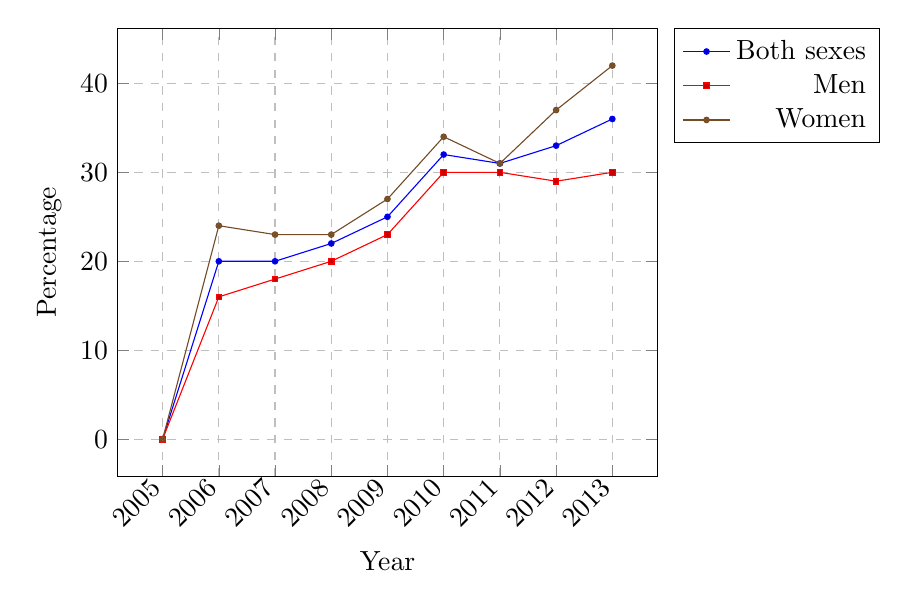
\begin{tikzpicture}
      \begin{axis}[
        xlabel={Year},
        ylabel={Percentage},
        legend style={cells={anchor=east}, legend pos=outer north east,},
        xtick=data,
        x tick label style={rotate=45, anchor=east, /pgf/number format/1000 sep=},
        mark size=1.0pt,
        grid=major,
        grid style={dashed},
      ]
      \legend{Both sexes, Men, Women}
      \addplot coordinates {
        (2005, 0)
        (2006, 20)
        (2007, 20)
        (2008, 22)
        (2009, 25)
        (2010, 32)
        (2011, 31)
        (2012, 33)
        (2013, 36)
      };
      \addplot coordinates {
        (2005, 0)
        (2006, 16)
        (2007, 18)
        (2008, 20)
        (2009, 23)
        (2010, 30)
        (2011, 30)
        (2012, 29)
        (2013, 30)
      };
      \addplot coordinates {
        (2005, 0)
        (2006, 24)
        (2007, 23)
        (2008, 23)
        (2009, 27)
        (2010, 34)
        (2011, 31)
        (2012, 37)
        (2013, 42)
      };
      \end{axis}
    \end{tikzpicture}
    \label{fig:ecommerce-in-norway}
    \caption{E-commerce purchases in Norway since 2005~\cite{statisticsNorway}}
  \end{figure}
}

\section{Motivation}
\label{sec:motivation}

% What are recommender systems good for?
In today's day and age the increasing amount of data overwhelm our human
processing capabilities in many information seeking tasks. To cope with this
overload researchers have introduced recommender system to filter the ever
increasing information and only present a small selection of items which
reflects the users tastes, interests and priorities. Recommender systems are an
active research field and has been successfully applied to many different
services ranging from e-commerce sites such as \emph{Amazon}, movie and
TV-series streaming services like \emph{Netflix} and in different music
applications such as \emph{Last.fm} and \emph{iTunes}.

% What is telenors incentive?
Many of the largest commerce Web sites have been using recommender systems to
help their customers find products to purchase for nearly two decades.
Schafer et al.~\cite{Schafer1999} identified three ways, in which recommender
systems increase E-commerce sales: (1) Browser into buyers: Recommender systems
can help customers find products they wish to purchase, (2) Cross-sell:
Recommender systems improve cross-sell by suggesting additional products for
the customer to purchase and (3) Loyalty: In a world where the competitor only
is one click away, gaining customer loyalty is an essential customer strategy.
Recommender systems improve loyalty by creating a value added relationship
between the site and the customer.

% What is the app and what makes it unique?
SoBazaar is a new \textit{fashion e-commerce application} for web and hand held
devices developed by Telenor, Norway's largest Telco company. The application
aggregates fashion products from various brands and stores into one \emph{news
feed} with recommended products, enabling the user to shop clothes and
accessories effortlessly and without the need of registering an account on
multiple web stores. Currently the application makes global recommendations
based on popular products and trends within social networks --- however, the goal
before launching the application this upcoming summer (\the\year) is to improve
these ratings making them personalized and grounded in a larger array of
features. This has as noted the potential of improving sales, activity and user
satisfaction.

% Discuss potential in fashion and e-commerce sales.
\ecommercenorway{}

The growth potential of such an application is immense in Norway. Numbers from
Statistics Norway~\cite{statisticsNorway} which are presented in the above
figure, shows a steady increase in the number of e-commerce sales of about 8\%
per year, from 2005. Still the competition, especially within personalized
recommendations, is insubstatial at both a national and international level, as
we will see in a detailed comptetitor analysis in
Section~\ref{subsec:competitors}. This underlines the importance of both the
discoveries made in this thesis and the application itself.

% Limited amount of data -> we need to utilize other sources. Implicit!
As the application is not yet officially released there is a limited amount of
user-item interaction from a set of beta users. In addition users do not have
the possibility to explicitly rate items on a numeric scale, a scheme often
employed by machine learning engineers and application developers in order to
understand their users preferences. Combining these two factors makes the
recommendation scenario both interesting and unique, since we need to utilize
the implicit information contained in user behavior such as clicking, wanting
or buying an item. Limited data both in number of users, but also in activity,
makes the system prone to what is called \textit{cold-start issues}, where
making recommendations with limited information is resolved by a variety of
techniques.

% The fashion domain have certain challenges.
This scenario differs from making recommendations on movies, books and music,
not just in the lack of rich explicit ratings, but also in the context of the
domain the recommendations will be done, namely the fashion domain. Firstly,
fashion consumption is largely determined by seasons. E.g. one does not buy
winter jackets in the middle of summer. Most clothes do also go out of
fashion, the same can not be said for \emph{all} movies. Secondly, there are a
whole different set of important aspects regarding the items or products when
recommending in the fashion domain, such as: brand, color and size.

% Brand and price are important!
Finally, users are highly price and brand-aware. This can be exemplified by
looking at an average movie consumer, where typically the director of the movie
does not greatly affect the way the movie is consumed. However, in the fashion
domain the consumer might mainly look at the product brand when deciding what
to consume. Price preferences are also related to this property where some
users prefer making \textit{a good deal} on periodic sales whilst other buys
clothes not only for individual satisfaction, but to show of or make a
statement.

% What are our goals and purpose?
In our system, there are two sources of information available for making
recommendations: an aggregated product database and event logs capturing user
activities. Out first goal is to find a technique for translating the implicit
feedback into preferences. These preferences are then combined with product
features and techniques for mitigating the cold-start problem. Finally the
user-item preferences are utilized in making recommendations where challenges
related to both domain and data sources are considered.

% Example scenario
For the users of SoBazaar the final product should not infer with the already
established user interface. Instead the news feed will evolve from today
showing the same recommendations to all users, to showing \textit{personalized
recommendations} to every user, based on their \textit{behavior} in the
application. For every user-item interaction the user is implicitly changing
his/hers preference-profile and will then, by just using the application, get
novel and more robust recommendations. Further, as personalized recommendations
hopefully will increase both sales and user activity we will, with a larger set
of data, be able to understand more user patterns and consequently gain a
deeper understanding of the domain.

\section{Problem Statement and Goals}

% Overall problem statement
The primary aim of this thesis is proposing a system, producing personalized
fashion recommendations based on user behaviour and product features, when both
resources are extremely limited in both quality and volume.

% Introduce goals related to domain
In order to propose such a system, one need a exhaustive understanding of both
the fashion domain and available data. In addition a study is required looking
at existing solutions, competitors and idientify potential competitive
advantages. Finally a discussion on how to overcome found challenges with
respect to both understanding the implicit feedback and making recommendations
is needed. Hence, our domain specific goals can be defined as:

% Domain-specific goals
\begin{itemize}
	\item \textbf{G1}: Gain a better understanding of the fashion domain.
  \item \textbf{G2}: Identify the specific challenges of making fashion recommendations.
  \item \textbf{G3}: Study how existing technologies can be adapted to mitigate or
  overcome these challenges.
\end{itemize}

% Introduce goals related to cold-start
In most recommender systems one base future recommendations on existing
feedback already given by the user. An important however is what to recommend
when no feedback has been given, which is the case for any new user. The same
issue is apparent when a new item is added to the application, where we need a
strategy for introducing it to users although the product is not connected to
any existing feedback. Finally, the closely related problem of making
recommendations in scenarios where feedback is extremely sparse need to be
addressed. First impressions are important both for retention and customer
satisfaction and consequently, seperate goals were set specifically concerning
cold-start issues.

\begin{itemize}
  \item \textbf{G4}: Study existing solutions to the cold-start.
  \item \textbf{G5}: Identify the best suited methods with regards to both application
  feedback and domain.
\end{itemize}

% Introduce goals related to implicit feedback
There is no explicit way for users to \textit{rate} or give \textit{negative
feedback} to items in SoBazaar. This forces us to look at user behaviour and
more specifically interactions on items such as \textit{clicking},
\textit{wanting} or \textit{purchasing}. We would like to learn how these
events could be used to predict the users true preferences. Using implicit
feedback yields the following goals:

\begin{itemize}
  \item \textbf{G6}: Explore the existing solutions of how to infer user preference from
  implicit feedback data.
  \item \textbf{G7}: Identify different methods of combining various event types into
  \emph{implicit ratings}.
  \item \textbf{G8}: Find metrics in order to evaluate the \emph{implicit ratings}.
\end{itemize}

% Introduce limitations
\paragraph{Limitiations} Our problem statement and consequent goals establish
the main theme of this thesis, but simultaneously they introduce some
limitiations. Hence, the reader should be familiar with what this thesis
\textit{does not set out to do}.

% Small and sparse dataset
The main limitiation of this thesis are primarly linked to having only one
available dataset with both sparse and modest data. As a result, making
conclusions based user behaviour proved difficult due to lack of statistical
significance on many observations. Limitiations in both time available and
number of existing users with sufficient activity made is also impossible to
conduct a thorough user study, which could confirm possible found user
patterns.

% No external sources of information (or weak quality)
In addition, as seen in the overview, external sources of information such as
social networks and trust-based networks are not considered --- as the dataset
provided did not warrant this. As the products in the SoBazaar application are
aggregated from multiple sources, and hence product databases, the quality of
information are notably diverse. Consequently, since extracting basic content
features different from product titles became close to impossible without large
engineering efforts, the \textit{main focus} does not lie on hybrid recommender
systems (combining content and user-based recommendations), although some work
is done in this area.

\section{Application Overview}

\begin{figure}[H]
  \centering
  \begin{tikzpicture}[
    % Manually overriden in most of the nodes :-)
    node distance=2.3cm,
    block/.style={
      rectangle,
      draw,
      thick,
      inner sep=5pt,
      align=center,
      rounded corners,
      minimum width=2cm,
    },
    % Special style for the social networks
    social/.style={
      draw=red,
      densely dotted,
    },
    % Box surrounding the data sources.
    dsbox/.style={
      draw,
      dotted,
      minimum height=1.2cm,
    }
  ]

  % Create nodes - first, data sources.
  \node(db)     [block] {Product DB};
  \node(social) [block,social, right of=db] {Social data};
  \node(log)    [block,right of=social] {Event log};

  % Our various 'systems'
  \node(coldstart) [block, below = 3.5cm of db] { Cold-start\\booster };
  \node(converter) [block, below = 3.5cm of log] { Implicit\\Converter };
  \node(recommender) [block, below = 2cm of coldstart] { Recommender };
  \node(evaluation) [block, right = 3.5cm of recommender] { Evaluation };

  % Box around data sources.
  \node (datasources) [dsbox, fit=(db) (social) (log)] {};
  \node at (datasources.north) [above, inner sep=2mm] {Data sources};

  % Draw the links between systems and data sources.
  \path[->,thick]
     (log) edge [] node [sloped, above] {Implicit feedback} (converter)
     (db) edge [] node [sloped, above, text width=3cm, align=center] {Structured\\product data} (coldstart)
     (converter) edge [] node [sloped, above] {Ratings} (coldstart)
     (coldstart) edge [] node [sloped, above] {Ratings} (recommender)
     (recommender) edge [] node [sloped, above] {Recommendations} (evaluation);

  \end{tikzpicture}
  \caption{Application overview, showing input and output from different
  components in the proposed system}
\end{figure}

\section{System Overview}

\marginpar{Include filterbots in a more detailed system overview?}

This thesis proposes a system for making recommendations based on implicit
data, where the input is implicit feedback collected on a set of users and
items and the output is personalized recommendations to all users, proposing
new and relevant products to their preferences.

\begin{figure}[H]
  \centering
  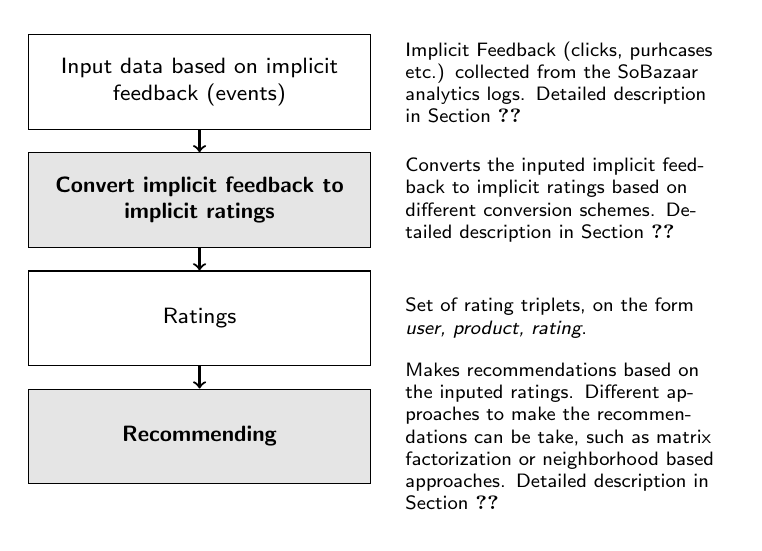
\begin{tikzpicture}
    [node distance = 1cm, auto,font=\footnotesize,
    % STYLES
    every node/.style={node distance=1.5cm},
    % The comment style is used to describe the characteristics of each process
    comment/.style={rectangle, inner sep= 5pt, text width=4cm, node distance=0.25cm, font=\scriptsize\sffamily},
    % The nonProcess style
    nonProcess/.style={rectangle, draw, inner sep=5pt, text width=4cm, text badly centered, minimum height=1.2cm, font=\footnotesize\sffamily},
    % The process style is used to draw the processs' name
    process/.style={rectangle, draw, fill=black!10, inner sep=5pt, text width=4cm, text badly centered, minimum height=1.2cm, font=\bfseries\footnotesize\sffamily}]

    % Draw processs
    \node [nonProcess] (inputData) {Input data based on implicit feedback (events)};
    \node [process, below of=inputData] (implicitConverter) {Convert implicit feedback to implicit ratings};
    \node [nonProcess, below of=implicitConverter] (ratings) {Ratings};
    \node [process, below of=ratings] (recommendations) {Recommending};

    \node [comment, right=0.25 of inputData] (comment-inputData) {
      Implicit Feedback (clicks, purhcases etc.) collected from the SoBazaar
      analytics logs. Detailed description in Section~\ref{sec:sobazaar-data}
    };

    \node [comment, right=0.25 of implicitConverter] (comment-implicitConverter) {
      Converts the inputed implicit feedback to implicit ratings based on
      different conversion schemes. Detailed description in
      Section~\ref{sec:implementation-implicit}
    };

    \node [comment, right=0.25 of ratings] (comment-ratings) {
      Set of rating triplets, on the form \textit{user, product, rating}.
    };

    \node [comment, right=0.25 of recommendations] (comment-recommendations) {
      Makes recommendations based on the inputed ratings. Different
      approaches to make the recommendations can be take, such as matrix
      factorization or neighborhood based approaches. Detailed description in
      Section~\ref{sec:making-recommendations}
    };

    % Draw the links between processs
    \path[->,thick]
      (inputData) edge (implicitConverter)
      (implicitConverter) edge (ratings)
      (ratings) edge (recommendations);

  \end{tikzpicture}
  \caption{Overview of the system. Boxes in white represents input and output
  data. Boxes in gray represents processes}
\end{figure}

Traditionally in most recommender systems this process does not include the
first two stages of our system, hence going directly from a set of explicitly
provided ratings to a set of recommendations. However, as we will see, making
ourselves non-dependent on explicit ratings can both provide us with a good
set of recommendations and take us one step closer to true artificial
intelligence, as we require no extra effort from the users --- rather learning
preferences from their behavior.

\section{Outline}
\begin{table}[H]
  \centering
  \begin{tabular}{lp{11cm}}
  \toprule
    \textbf{Chapter}      & \textbf{Description} \\
  \midrule

    Chapter \ref{chap:introduction} & The~\nameref{chap:introduction} chapter gives an overview of the
    project to the reader. It also outlines the purpose and motivation of the
    project.  \\[1.5ex]

    Chapter \ref{chap:thesobazaardata} & \nameref{chap:thesobazaardata} chapter presents the results from our
    dataset analysis. \\[1.5ex]

    Chapter \ref{chap:SotA} & The \nameref{chap:SotA} chapter documents knowledge,
    research and technology that are relevant to the project, and how and why
    some of them were prioritized over others when it comes to how they are
    used in the project. \\[1.5ex]

    Chapter \ref{chap:implementaion} & The \nameref{chap:implementaion} chapter describes the design of the
    system and how the design has been implemented. \\[1.5ex]

    Chapter \ref{chap:resulteval} & The \nameref{chap:resulteval} chapter discus the development process,
    testing of results and major issues. \\[1.5ex]

    Chapter \ref{chap:conclusion} & The \nameref{chap:conclusion} chapter sums up the project and describes the
    findings and reflects on them. It also describes further work.
    \\[1.5ex]

    Appendix & \textbf{The Appendix} contains extended information such as a full list of the requirements. \\

  \bottomrule
  \end{tabular}
  \caption{Overview of structure and chapters in the thesis}
  \label{table-reportstructure}
\end{table}

% !TEX root = ../report.tex

\chapter{Preliminary Study}
\minitoc

\clearpage

\section{State Of The Art}
\subsection{System Coldstart Handling}
\subsection{Fashion Recommendation}
\subsection{Session Based Recommendation}
Articles 4 l8er:
In Proceedings Of
the 1995 International Joint Conference on Artificial Intelligence, 1995. Montreal,
Canada.

S. Schechter, M. Krishnan, and M. D. Smith. Using path profiles to predict http
requests. In Proceedings of 7th International World Wide Web Conference, Novem-
ber 1998. Brisbane, Australia.

M. Spiliopoulou and L. C. Faulstich. Wum: A web utilization miner. In In Pro-
ceedings of EDBT Workshop WebDB98, 1999. Valencia, Spain.

R. Cooley, B. Mobasher, and J. Srivastava. Data preparation for mining world wide
web browsing patterns. Journal of Knowledge and Information Systems, 1(1), 1999.

B. Mobasher, H. Dai, T. Luo, and M. Nakagawa. Discovery of aggregate usage
profiles for web personalization. In Proceedings of the Web Mining for E-Commerce
Workshop (WebKDD’2000), 2000.

C. Shahabi, A. Zarkesh, J. Adibi, and V. Shah. Knowledge discovery from users
web-page navigation. In Proceeding of the IEEE RIDE97 Workshop, pages 20–29,
April 1997. Birmingham, England.

O. Nasraoui, R. Krishnapuram, and A. Joshi. Mining web access logs using a fuzzy
relational clustering algorithm based on a robust estimator. In Proceedings of Eight
International World Wide Web Conference, 1999. Toronto, Canada.

Y. Yan, M. Jacobsen, Garc ̈ıa-Molina H, and U. Dayal. From user access patterns to
dynamic hypertext linking. In Proceedings of the Fifth International World Wide
Web Conference, 1996. Paris, France.

A. Nanopoulos, D. Katsaros, and Y. Manolopoulos. Effective prediction of web-
user accesses: a data mining approach. In Proceedings of WEBKDD workshop,
2001. San Francisco, CA, USA.

R. Agrawal and R. Srikant. Mining sequential patterns. In Proceedings of the In-
ternational Conference on Data Engineering (ICDE), March 1995. Taipei, Taiwan

M. Deshpande and G. Karypis. Selective markov models for predicting web-page
accesses. In Proceedings of the First SIAM International Conference on Data Min-
ing (SDM’2001), 2001.

R. R. Sarukkai. Link prediction and path analysis using markov chains. In Proceed-
ings of the Ninth International World Wide Web Conference, 2000. Amsterdam.


%http://dl.acm.org/citation.cfm?id=1136004
%http://link.springer.com/chapter/10.1007/3-540-46119-1_42
%http://dl.acm.org/citation.cfm?id=1082567
%http://link.springer.com/chapter/10.1007%2F978-3-540-30214-8_20
%http://dl.acm.org/citation.cfm?id=502935
%http://dl.acm.org/citation.cfm?id=1835896
%http://dl.acm.org/citation.cfm?id=345169
%http://dl.acm.org/citation.cfm?id=345169

\subsection{Recommenders (Similar systems? somethingsomething)}

\section{Data Findings}
\subsection{What Can Be Understood From The Data}
\subsubsection{The Expected}
Event "app_started"; all have user_id's
Event "app_first_started"; all user_id's are NULL
Event "user_logged_in"; all have user_id's... (assigned with login, event saved after login?)

\subsubsection{The Strange}
NULL valued events: (Not all strange, but put together for readability)
facebook_share_changed
collection_viewed
wantlist_menu_entry_clicked
app_became_active

app_first_started
facebook_login_failed

> db.prod.distinct('event_json.ipAddress').length
9033
> db.prod.distinct('event_json.eventData.device_id').length
2644
> db.prod.distinct('user_id').length
1660

More devices than users, can't fill the blanks with device_id

\subsection{Graphs N' Shit}

\section{What to use}
\subsection{Some Awesome Algorithms (Build up with project progress)}
\subsubsection{The Good}
\subsubsection{The Bad}
\subsection{Why Not To Use These (Same As above)}
\subsubsection{The Good}
\subsubsection{The Bad}

\section{How to evaluate}
\subsection{What Has Been Done Before}
\subsection{What To Use}
\subsubsection{The Good}
\subsubsection{The Bad}

\section{Evaluation}

% !TEX root = ../report.tex

\chapter{Requirements}
\minitoc

\clearpage

\section{Capturing the Requirements}

\section{Functional Requirements}\label{section:functional-requirements}
\begin{description}
  \item[FR1]
  \item[FR6]
  \item[FR7]
\end{description}

\subsubsection{FR1}

\subsubsection{FR6}

\subsubsection{FR7}


\section{Non Functional Requirements}\label{section:non-functional-requirements}
\begin{description}
  \item[NFR1]
\end{description}

\subsubsection{NFR1}


\section{Prioritized Requirements}

% !TEX root = ../report.tex

\chapter{Implementation}
\label{chap:implementaion}
\minitoc

\clearpage

% !TEX root = ../../report.tex
\section{Generating Implicit Ratings}
\label{sec:implementation-implicit}

In this section we continue solving the problem of generating ratings based on
implicit feedback found in analytics logs, as defined in
Section~\ref{sec:implicit}. Our goals are two-fold:
% TODO: Reference research goals
\begin{itemize}
  \item Find novel ways of creating implicit ratings, remedying as many
  weaknesses and challenges, depicted in Section~\ref{implicit-weaknesses}, as
  possible
  \item Customize existing and new algorithms to our fashion domain, described
  in Section~\ref{sec:fashion}
\end{itemize}

The most important factor when creating ratings is to understand which implicit
data are available and their implications on user preferences. In order to best
understand the data one should do a quantitative study as presented in
Chapter~\ref{chap:thesobazaardata}, but always keeping in mind the domain in question.
When an understanding is obtained one can begin selecting features capturing
the wanted properties and use these generalizations in order to generate
ratings for different users inhabiting unique patterns and product
interactions.

Then, upon evaluation of conversion features we can do an initial analysis
without any metrics by attempting to answer the question \textit{does this
generalization capture the domain and data properties?}
One such generalization, often done, is counting the number of a specified
activity on an item, correlating it with preference. In the case of SoBazaar
we've seen that a higher number of clicks yields a higher probability of
purchasing an item, thus we can use the number of clicks as a feature in
generating ratings - correlating a higher number of clicks to a higher rating.

Other properties, which we will discuss in this section and consequently
utilize, found in the \textit{fashion store aggregation} domain are:

\begin{itemize}
  \item Items have a short lifespan, due to:
  \begin{itemize}
    \item Seasons
    \item Fashion and trends
    \item Sales and price fluctuations
  \end{itemize}
  \item Items are not bought regularily, as with food and other convenience
  products
  \item Users are cost and brand-aware
\end{itemize}

Given a good set of chosen features we should, for all users that have
interacted with various items, obtain a well-distributed list of ratings - and
with more implicit feedback available for a user, we should obtain a higher
probability of the user having an unique set of ratings. This is easily seen in
the scenario where we do not consider social-graphs between users, and we have
two users $u_1$ and $u_2$ who has the equal implicit feedback - e.g. they
viewed the same items. If we only use global features, such as item popularity,
we have no way of giving unique ratings to the two users. However, if we
instead look at user-features such as \textit{when} did the users last look at
the items and \textit{in which order}, we have a higher probability of
obtaining unique sets of ratings.

When ratings are not explicit, the implicit ratings becomes the recommender
systems equivalent of a ground truth and all later stages in the recommender
pipeline (See Section~\ref{sec:app-overview}) are dependent on the ratings representing a users
preferences. This highlights the importance of generating high quality ratings
and selecting good features and methods for doing so.

\subsection{Improving mapping of event types}

In Section~\ref{implicit-binary-domains} Pranab Ghosh proposes a global rating
mapping without any specific justification of why the different values are
chosen~\cite{pkghost2014implicit}. In order to use this method we wanted our
weighting of various events to be grounded in statistical properties found in
the dataset. Further we would like to create ratings on a continuous scale
between a min and max-value for the given event, not manually define levels of
scores. This way we could use a \textit{penalization function}, that based on
our selected feature ensured an even distribution between the minimum and
maximum value for the event in question. For example giving an often clicked
product for a user the maximum value and conversely the minimum value for
infrequent clicks.

To select good weights we thus considered the probability of each event that we
wanted to base our ratings on. These events were the ones having a
\textit{product id} as well as possibly inhabiting the implicit properties
described above. Instead of manually map events to an arbitrary score we used
the probability obtaining the given event type, given all events. Thus, our
score mapping looks like:

\begin{table}[H]
  \centering
  \begin{tabular}{llll}
    \toprule
      Event type & Probability & Min ($m_e$) & Max ($M_e$) \\
    \midrule
      \textit{product\_detail\_clicked}     & $\frac{21400}{35324} \approx 61$  & 0   & 61  \\[1.5ex]
      \textit{product\_wanted}              & $\frac{12436}{35324} \approx 35$  & 61  & 96  \\[1.5ex]
      \textit{product\_purchase\_intended}  & $\frac{1488}{35324} \approx 4$    & 96  & 100 \\
    \bottomrule
  \end{tabular}
\end{table}

Notice that the total number of events having a product id is 40686, and the
sum of all three fractions is 1, thus covering 100\% of all events.

\subsection{Penalizing features}

How then do we distribute the feature-values  between the min and max limits
above? In our first implementation we use a \textit{linear penalization}
function, set in such a way that $0 \leq p(x) \leq 1$ and $0 \leq x \leq F_u$
where $F_u$ is the maximal observed value for user $u$ of the feature in
question, defined as:

\begin{equation}
  p(x, u) = \frac{x}{F_u}
\end{equation}

By considering penalization we also implicitly add negative feedback to events.
This is an important aspect to keep in mind when working with implicit
feedback, as discussed in Section~\ref{sec:implicit} as modern recommender
engines work better when we are assuming ratings are based on both positive and
negative feedback.

Given $p(x, u)$ we formalize an equation for finding $S_e(x, u)$, the score
given to event $e$ after penalization, given a max $M_e$ and min $m_e$ value.

\begin{equation}
  S_e(x,u) = M_e - (M_e - m_e) \cdot p(x, u)
\end{equation}

The last component needed is normalizing the ratings. Which is described in
Equation~\ref{eq-normalization}. And now we have all components ready in order
to do a rating generation.

\subsection{Considering recentness}

In order to see all parts working together, we imagine an example where a user
has six events on three items, as presented in the table below. The ratings are
normalized between 1 and 5 and the product IDs are there for illustrative
purposes. We choose to look at the number of days since the user did the event
in question as the implicit feature, where $x=0$ means the event was registered
today (or as the most recent) and in our example $x=14$ is the oldest event
happening two weeks ago, hence $F_u = 14$.

\begin{table}[H]
  \centering
  \begin{tabular}{llllll}
  \toprule
  Event type & Product ID & x (days) & p(x) & Score & Rating \\
  \midrule
  \textit{product\_purchase\_intended}  & 1 & 0   & $\frac{0}{14} = 0.00$  & 100 & 5.00 \\[1.5ex]
  \textit{product\_purchase\_intended}  & 2 & 3   & $\frac{3}{14} = 0.21$  & 98.95 & 4.96 \\[1.5ex]
  \textit{product\_wanted}              & 2 & 7   & $\frac{7}{14} = 0.50$  & 78.5 & 4.14 \\[1.5ex]
  \textit{product\_detail\_clicked}     & 1 & 0   & $\frac{0}{14} = 0.00$  & 62 & 3.48 \\[1.5ex]
  \textit{product\_detail\_clicked}     & 3 & 7   & $\frac{7}{14} = 0.50$  & 31 & 2.24 \\[1.5ex]
  \textit{product\_detail\_clicked}     & 2 & 14  & $\frac{14}{14} = 1.00$ & 62 & 1.0  \\
  \bottomrule
  \end{tabular}
  \caption{Showing penalizations and ratings on example data}
  \label{implicit-ratings-example}
\end{table}

When finally selecting a rating for the user/product pair, we choose the
one yielding the highest value for the given product. Hence for the three items
with IDs 1, 2 and 3 above we obtain the ratings 5.00, 4.96 and 2.24, respectively.

Using the same method on the SoBazaar dataset yields the following distribution
of ratings, where we group ratings together into 150 different bins - thus
every bin having an interval size of 0.0267:

\begin{figure}[H]
  \centering
  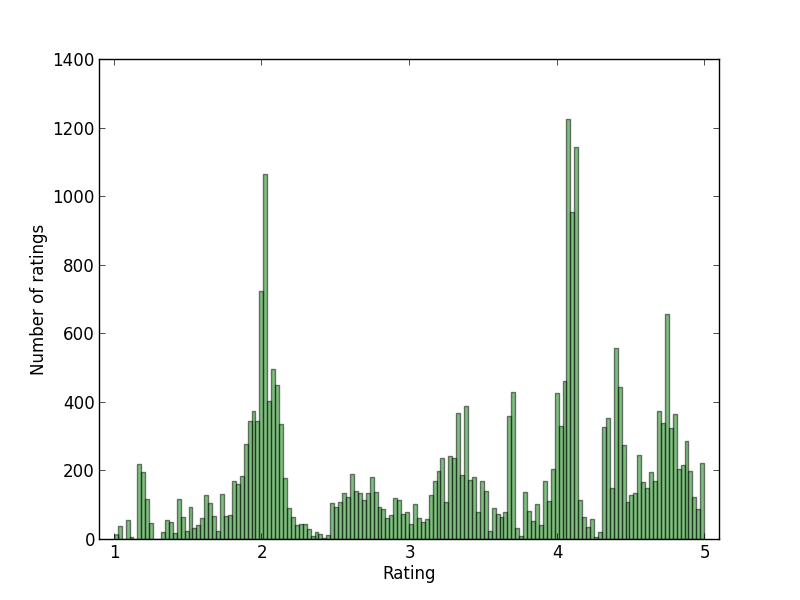
\includegraphics[scale=0.6]{image/dist-recentness-linear-global}
 \caption[Distribution of ratings using number of days since event]{Distribution of ratings using number of days since event, a linear
 penalization function and global min/max feature-values}
  \label{fig:dist-recentness-linear-global}
\end{figure}

Worth noting is that we here use $F_u$ oldest event globally, and not per user,
since too many users only have one or two events, as per
Figure~\ref{fig:ratingsPerUser}. The average rating is \textit{3.29} with a
median \textit{3.37}. The weakness in these results however is easy to spot
given the scenario when a user is absent from the application over a longer
time and then returns. In this scenario all the items the user has previously
looked at, wanted or bought will all suffer from large penalization values -
and hence low ratings, since the x for all items is very high. In addition the
method does not scale well, unless one limit the $M_u$ value, so that the
difference between two adjacent x values are significant. As SoBazaar is a
relatively new application this proved not to be a problem with our
experiments, but given a larger dataset with older events we would recommend
testing $M_u = \min(O_e, L)$ where $O_e$ is the number of days since the oldest
event and $L$ is the limit, set at e.g. 200.

In order to mitigate the returning user problem we adjust our feature to
instead consider the ordering of events for user $u$. This way, given $n$
events registered for this user, the newest event would obtain $x=0$ and the
oldest $x=n$. We continue to use a linear penalization function, which yields
the following distribution:

\begin{figure}[H]
  \centering
  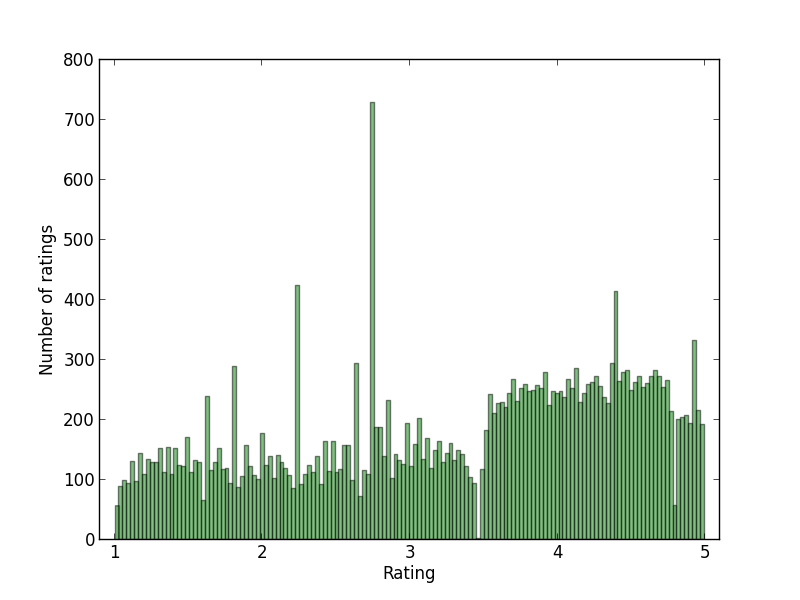
\includegraphics[scale=0.6]{image/dist-count-linear}
  \caption{Distribution of ratings using ordering of events, and a linear
 penalization function}
  \label{fig:dist-count-linear}
\end{figure}

With much the same average and median values at \textit{3.26} and \textit{3.45}
respectively, we still have a distribution with a unique pattern where the
ratings are more evenly distributed (the largest bin contains 700 ratings in
the given interval, compared to Figure~\ref{fig:dist-recentness-linear-global}
where the same number is 1250.)

\subsubsection{Penalization with logistic functions}

So far we've seen ratings generated by looking at the event recentness,
capturing important factors such as items having a short life-time and users
frequently shopping for different occasions and hence different types of
clothes. However, we want to improve the penalization function in order to
capture the following properties in our domain:

\begin{itemize}
  \item Recent events should count more towards a good rating, compared to old
  events.
  \item Seasons change at a fixed interval, and clothes goes out of season in
  the matter of weeks.
  \item A user may look at multiple clothes at once, comparing them and finding
  them all quite interesting.
\end{itemize}

When using a linear function the difference in penalization between the two
most recent items are equal to the difference between the oldest two items.
However, intuitively we consider a user to have multiple relevant items
concurrently and we know that in domains such as technology, fashion and other
consumer-products an item has an age of relevancy, somewhat metaphoric to a
seasonal threshold. An example of this could be a fashion store recommending
warm clothes in the months between December to March, but then want to "change"
product pool based on the users behaviors -- who are probably looking for
lighter clothes (changing season).

In order to mimic this behavior we introduce a logistic function, which is a
mathematical function having an "S" shape and a common special case of the more
general sigmoid-function. In its most simplest case the logistic function is
defined as:

% Vertical alignment of equation and plot.
\begin{figure}[H]
  \centering
  \noindent\begin{minipage}{.45\textwidth}
    \begin{tikzpicture}
      \begin{axis}
      \addplot[black,xlabel=$x$,ylabel=$f(x)$] {1/(1+exp(-x))};
      \end{axis}
    \end{tikzpicture}
  \end{minipage}
  \begin{minipage}{.45\textwidth}
  \begin{align}
    \label{logistic-function}
    f(x) = \frac{1}{1+\exp^{-x}}
  \end{align}
  \end{minipage}
  \caption{Logistic function having a S-shape with y-values ranging
  from 0 to 1.}
\end{figure}

Here the value of $f(x)$ is asymptotically limited between 0 and 1, dependent
on the value of $x$. The steepest point of the curve happens when $x=0$. By
adjusting the exponent of $e^{(-x)}$ we can skew the curve in order to map to our
data, giving us a \textit{function of relevancy} ranging from an item being
very relevant ($f(x)=0$) and not relevant ($f(x)=1$).

By adding two variables to the logistic function we can fine tune both the
steepness and range of $f(x)$. Hence we adjust Equation~\ref{logistic-function}
to include $s$, the \textit{steepness coefficient}, and $c$, the \textit{shift
coefficient}.

\begin{equation}
  p(x) = \frac{1}{1+\exp^{-s(x - c)}}
\end{equation}

In the standard sigmoid function these are $1$ and $0$ respectively, but by
adjusting $s$ closer to 0 we decrease the steepness, creating a more gradual
curve. Setting the $c$ to a larger number we shift the steepest point of the
curve to $x=c$, hence if we set $c$ to $20$, the steepest point (largest
acceleration) in our curve would be located when $x=20$.

We can manually try to set the steepnes and shift coeffiecients based on the
behaviour seen in the dataset provided. Using the data provided in
Table~\ref{implicit-ratings-example} we can again try to calculate the ratings
and penalizations. We set the steepness coefficient to be $0.8$, thus having a
curve that is not too steep yielding a good distribution. This constant works
well when the shift coefficient is low ($c \lessapprox 10$), however if the
shift coefficient increases the steepness should decrease. In our dataset we
found finding a fixed ratio between the steepness and shift worked best. The
shift is set at $M/2$, where $M$ equals the number of days between the oldest
and most recent event, in our example equalling 7.

\begin{table}[H]
  \centering
  \begin{tabular}{llllll}
  \toprule
  Event type & Product ID & x (days) & P(x) & Score & Rating \\
  \midrule
  \textit{product\_purchase\_intended}  & 1 & 0   & $\frac{1}{1 + \exp^{-0.8(0*7)}} = 0.00$  & 100 & 5.00 \\[1.5ex]
  \textit{product\_purchase\_intended}  & 2 & 3   & $\frac{1}{1 + \exp^{-0.8(3*7)}} = 0.03$  & 99.85 & 4.99 \\[1.5ex]
  \textit{product\_wanted}              & 2 & 7   & $\frac{1}{1 + \exp^{-0.8(7*7)}} = 0.50$  & 78.5 & 4.14 \\[1.5ex]
  \textit{product\_detail\_clicked}     & 1 & 0   & $\frac{1}{1 + \exp^{-0.8(0*7)}} = 0.00$  & 62 & 3.48 \\[1.5ex]
  \textit{product\_detail\_clicked}     & 3 & 7   & $\frac{1}{1 + \exp^{-0.8(7*7)}} = 0.50$  & 31 & 2.24 \\[1.5ex]
  \textit{product\_detail\_clicked}     & 2 & 14  & $\frac{1}{1 + \exp^{-0.8(14*7)}} = 1.00$ & 62 & 1.0  \\
  \bottomrule
  \end{tabular}
  \label{implicit-ratings-example-sigmoid}
\end{table}

Notice how the purchase of product with ID 2 went from $4.96$ in
Table~\ref{implicit-ratings-example} to $4.99$ here, as we have lower
penalization for lower x-values. Equally, the penalizations are equal ($0.50$
and $1.00$) when the x-values are 7 and 14 respectivly. However, while this
works fine in the example above we need to set the ratio between the steepness
and shift coefficient, as manually setting the steepness based on the
shift-coefficient is imprecise and non-scientific. Instead we alter our
logistic function to instead using a ratio $r$ between the two constants:

\begin{equation}
  p(x) = \frac{1}{1+e^{-(r/c) \cdot (x - c)}}
\end{equation}

Here the $c$ equals the steepest point (shift coefficient), and we set it so
that $c = M/2$ where $M$ still being the oldest event globally, as described in
the previous section. In the SoBazaar dataset $M$ was $224$. Using a different
ratio changes the logistic function in the following way:

\newcommand{\sigmoidfixed}[3]{
  % Draws a sigmoid-function.
  % #1 = ratio
  % #2 = max value
  % #3 = scale of image
  \begin{tikzpicture}[scale=#3]
    \begin{axis}[
      ymin=0,ymax=1,
      xmin=0,xmax=#2,
      grid=both,
    ]
    \addplot[
    black,
    xlabel=$x$,
    ylabel=$f(x)$,
    domain=0:#2]
    {1/(1+exp(-(#1/(#2/2))*(x-(#2/2))))};
    \end{axis}
  \end{tikzpicture}
}

\begin{figure}[H]
  \centering
  \begin{subfigure}[b]{0.3\textwidth}
    \sigmoidfixed{2.5}{235}{0.5}
    \caption{$r = 2.5$}
  \end{subfigure}
  \begin{subfigure}[b]{0.3\textwidth}
    \sigmoidfixed{3.5}{235}{0.5}
    \caption{$r = 3.5$}
  \end{subfigure}
  \begin{subfigure}[b]{0.3\textwidth}
    \sigmoidfixed{4.5}{235}{0.5}
    \caption{$r = 4.5$}
  \end{subfigure}
  \caption{Penalization functions for various ratios controlling steepness and
  shift}
  \label{fig:sigmoid-penalizations}
\end{figure}

As we want a good distribution, but still not penalize most recent items
linearly we choose a ratio of $3.5$ for our dataset, which creates the
distribution seen below. Tests were also carried out verifying that this was a
good selection.

\begin{figure}[H]
  \centering
  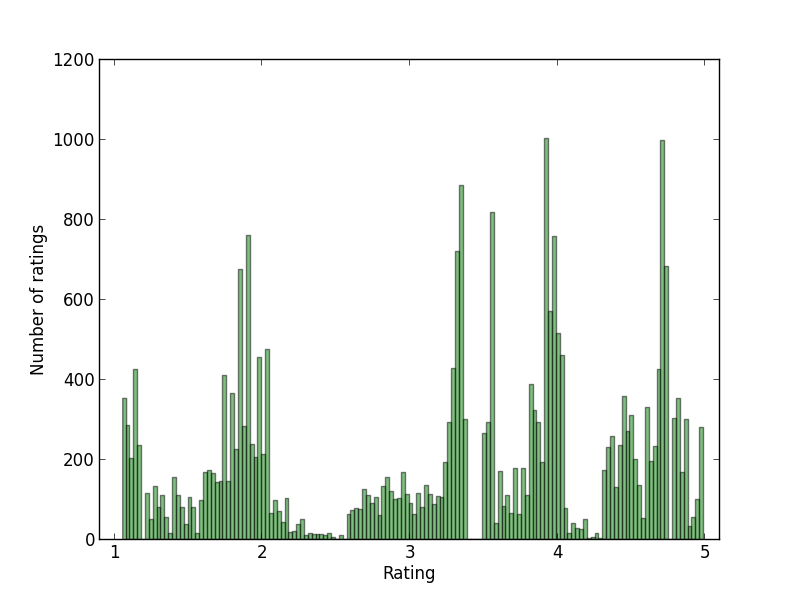
\includegraphics[scale=0.5]{image/dist-sigmoid-fixed-recentness-3-5}
  \caption[Distribution of ratings using number of days since earliest event]{Distribution of ratings using number of days since earliest event,
  a logistic penalization function and global min/max feature-values}
  \label{fig:dist-recentness-sigmoid}
\end{figure}

As discussed in the previous section, using number of days since most recent
event has many weaknesses, most notably the returning user - who if absent for
a longer time finds all items previously viewed or bought heavily penalized.
Instead we can use the ordering of items with a logistic penalization function
as well. Continuing with a ratio of $3.5$ we obtain the following distribution:

\begin{figure}[H]
  \centering
  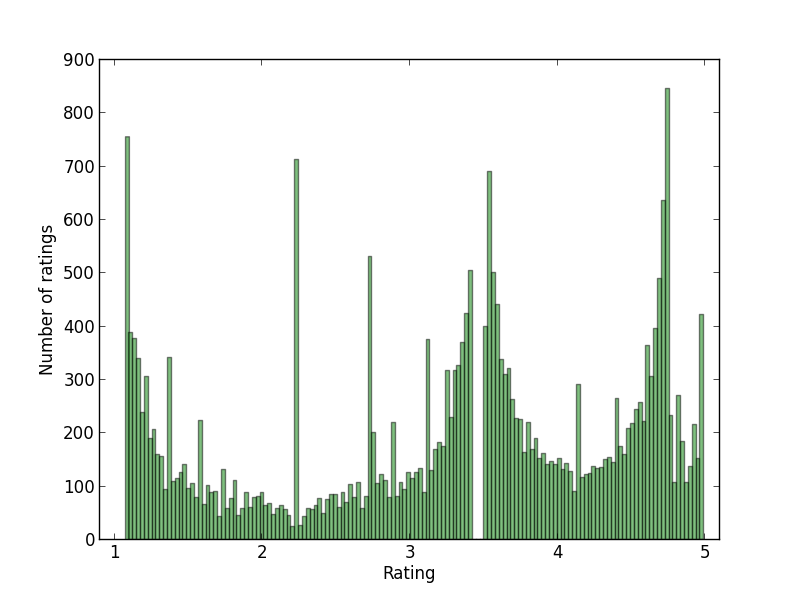
\includegraphics[scale=0.5]{image/dist-sigmoid-fixed-count-3-5}
  \caption[Distribution using ordering of events w/logistic penalization]{Distribution using ordering of events, a logistic penalization
  function and global min/max feature-values}
  \label{fig:dist-count-sigmoid}
\end{figure}

\subsection{Considering price}

In the same manner as with recentness we want to consider other features
apparent in our data and domain. As seen in Figure~\ref{fig:priceperUserDist} there is, not
surprisingly, a difference between users in average price on items they
frequent. Utilizing this variance we can create personalized ratings where we
try to give high ratings to items in the same price class as the user,
penalizing products that are too expensive or cheap.

The procedure is done in two steps: first we find the average price $a_u$ on
all items related to the user $u$. In the second step we make a second pass
over all items the user has shown interest in and calculate the distance to
$a_u$, yielding $x = p_i - a_u$ where $p_i$ is the price of item $i$. We then
find the penalization by:

\begin{equation}
  p(x,u) = \min{1, \frac{x}{M}}
\end{equation}

where $M$ is a constant controlling at which point the difference in price
should be fully penalized. In our experiments setting $M = 1500$ worked well,
hence making a price difference of $1500$ or more fully penalized yielding a
rating of 1.

Before applying the penalization function we make the assumption that an item
having the price difference $x = -d$ (cheaper) should be penalized less than an
item with the price difference $x = d$ (more expensive). Further we want to
make the value $x$ absolute, before calculating the penalization since $0 \leq
p(x,u) \leq 1$. In conclusion we apply $x = |\frac{x}{2}|$ $\text{if}$ $ x < 0$
making cheaper items half as sensitive to penalization, compared to more
expensive items.

\begin{figure}[H]
  \centering
  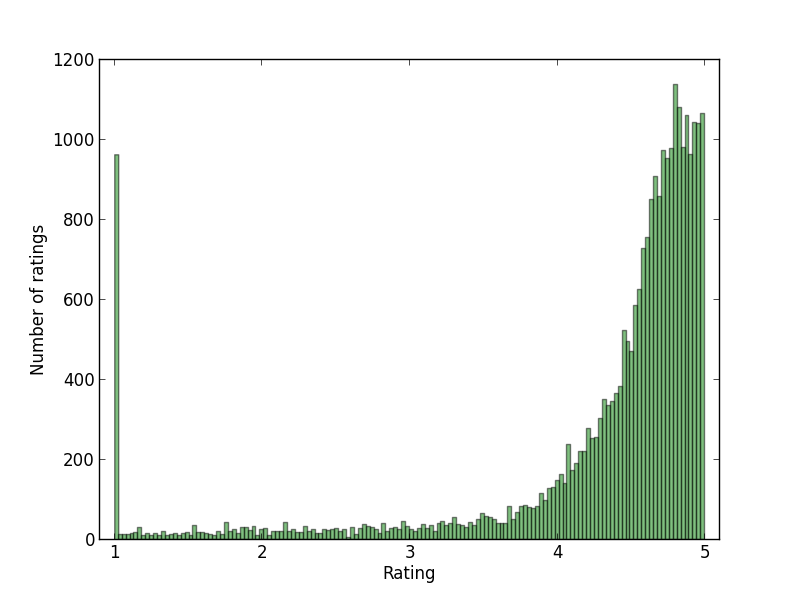
\includegraphics[scale=0.5]{image/dist-price}
  \caption{Distribution considering item price differences and each users conformity to
  its average price}
  \label{fig:dist-price}
\end{figure}

As seen the many items are penalized heavily for being to expensive, but this
is by design as we do not want to show too expensive items to the user
according to our assumptions. By setting $M$ higher, the number of items with
rating $1$ can be reduced. In addition most items gets a rating $5$ which tells
us that many users share the price preferences and by penalizing harder we can
reduce the number of items with rating 5. However, as we will see in subsequent
sections we are quite happy with the above distribution.

\subsection{Considering item popularity}

By looking at the global popularity of all item we can essentially tell if a
users activities classifies as conforming to the common standards or if the
users event patterns are more \textit{unique}. Our goal is to first classify to
which degree a user like globally popular items and then give penalizations to
items that are \textit{too popular} (the user is not adhering to peer-pressure)
or \textit{too obscure} (the user prefers popular items).

By first sorting all products by the number of related events we assign
a popularity score $0 \leq p \leq 1$, where $p=0$ is the product with the most
events and $p=1$ the event with the least number of events. Then we calculate
the average popularity score $a_e$ across all events, yielding $a_e = 0.76$.

In order to find a good penalization function we looked for the following
properties:

\begin{itemize}
  \item The top-value of $y$ should be at $x = 0.76$.
  \item When $x = 0$, that is for the most popular item, we should not penalize
  with $1.0$ nor $0.0$. A value of $y = 0.5$ was chosen.
  \item At $x = 1$ we want $y = 1$, giving maximum penalization to
  inpopular items.
\end{itemize}

And settled for having two linear functions, one when the popularity of item
$i$ was below the average popularity ($p_i < a_e$) and the second for when the
popularity was equal or higher.

\begin{equation}
  p(x, u) =
    \begin{cases}
      -\frac{c}{a_e}x + c                     & \text{if } x < a_e \\[1.5ex]
      \frac{1}{1-a_e}x - \frac{1}{1-a_e} + 1  & \text{if } x \geq 0
    \end{cases}
\end{equation}

where $c$ is the value chosen as penalization to the most popular item. As
mentioned this was in our experiments set to $0.5$. Using the SoBazaar $a_e$ we
obtained the following distribution and penalization function after
normalization:

\begin{figure}[H]
  \begin{subfigure}[b]{0.56\textwidth}
    \centering
    \resizebox{\linewidth}{!}{
      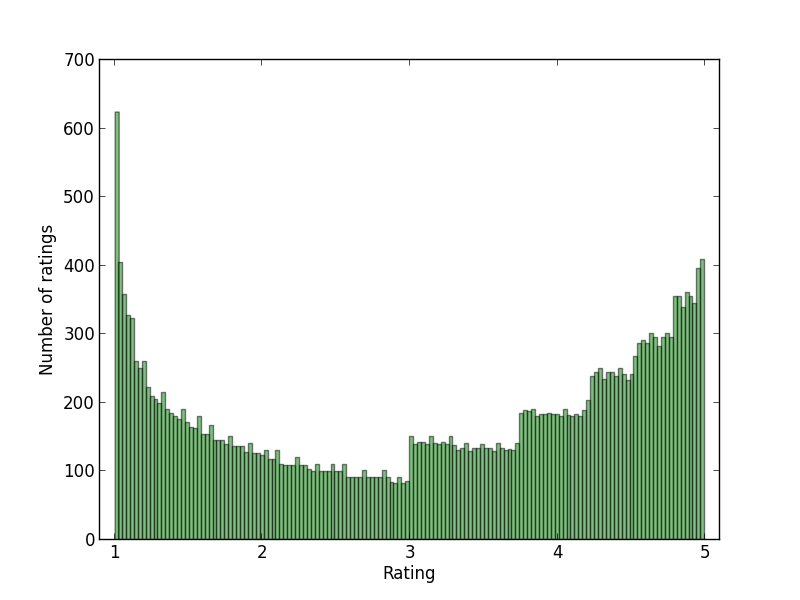
\includegraphics{image/dist-popularity}
    }
  \end{subfigure}
  \begin{subfigure}[b]{0.5\textwidth}
    \centering
    \resizebox{\linewidth}{!}{
      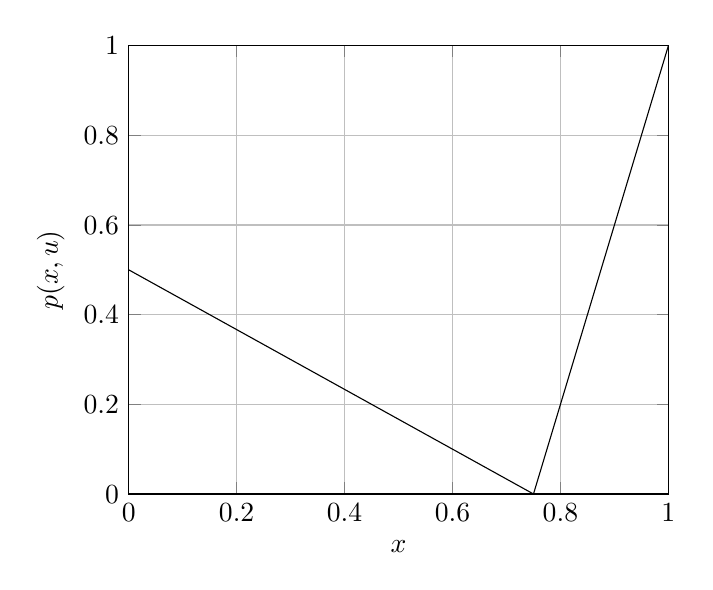
\begin{tikzpicture}
        \begin{axis}[
          ymin=0,ymax=1,
          xmin=0,xmax=1,
          grid=both,
          xlabel=$x$,
          ylabel={$p(x,u)$}
        ]
          \addplot[black] {-0.5/0.75*x + 0.5};
          \addplot[black] {1/(1-0.75)*x - 1/(1-0.75) + 1};
        \end{axis}
      \end{tikzpicture}
    }
  \end{subfigure}
  \caption[Distribution of popularity based ratings]{Distribution and penalization function, considering item popularity
  and the users conformity to popular items}
  \label{fig:dist-popularity}
\end{figure}

The peak at rating $1$ is a result of many items having close to zero events
connected to them. More interestingly we observe an evenly distributed spread
of ratings and, as with price, a peak at rating $5$ is expected as this is
given to the items close to the \textit{average} popularity.

\subsection{Linearly combining implicit ratings}

At this point we have found multiple ways of calculating the implicit ratings,
based on our implicit feedback. However, each method has its weaknesses,
strengths and captures different feature-sets in our data. Thus the
distributions reflect a large difference in ratings. Selecting a feature such
as number of days since the event in question captures our implicit knowledge
about seasons and items having a short life-span. However, as pointed out
earlier given many events on the same day there are no way of differentiating
them - unless we consider the ordering of items, saying the most recent item
shall be higher rated than older events. However, exclusively changing the
feature like this forces us to loose some of our implicit data about items
having a fixed lifespan. What we want to do is \textit{combine the two
features} in a procedure that often in recommender systems are coined
\textit{blending} or \textit{ensemble methods}. Combining them enables us to
create more robust ratings where weaknesses such as outliers or inconsistencies
in one method can be averaged out by the strengths of others. If two features
independently finds the same properties and ratings for some items and users,
then the result and our belief is strengthened.

When linearly combining $M$ models $m_1 \dots m_M$, we choose $M$ factors $f_i$
all adding up to 1.0, representing the weight of model $m_{i}$ in the final
\textit{blend}. Each model then have $k$ ratings on the triplet form
\textit{(user, product, rating)} and noted noted as $r_{ij}$ - the rating of
item $j$ in model $i$.

Then when calculating the final rating for item $j$ we sum over all
models:

\begin{equation}
  r_j = \sum _{i=1}^{M} f_{i} * r_{ij}
\end{equation}

Given two models, we can observe the result of performing a blend between with
factors $f_1 = 0.7$ and $f_2 = 0.3$ and the two ratings $r_{11} = 5$ and
$m_{21} = 3$ for a given item, we can calculate the final rating as $(0.7
\times 5) + (0.3 \times 3) = 4.4$. The obvious weakness in this approach is the
need for manually setting weights for $M$ different factors. Optimally we would
like to run one blend, look at the result, compare it to previous results and
make adjustments to the weights based these. This is what is done in simple
blending schemes using Linear Regression or KNN, but many state-of-the-art
schemes exists as well such as Binned Linear Regression, Bagged Gradient
Boosted Decision Tree (BGBDT), Neural Networks and Kernel Ridge Regression
Blending \cite{jahrer2010combining} \cite{toscher2009bigchaos} which are based
on the same principles.

However, as discussed in Section~\ref{sec:implicit}, when creating ratings from implicit
feedback we lack a ground truth -- that is we make several assumptions on which
implicit features contribute towards higher preference and thus higher ratings,
but with no real means of confirming the assumptions. A user buying an item as
a gift for a friend may not actually like the item and would not give a high
rating - and this, with a traditional collaborative filtering approach based on
explicit feedback would be accounted for, looking at the user pattern of the
user and labeling the purchase as an outlier. Without this ground truth however
we can not without injecting negative feedback, based on assumptions, make
classifications of outliers nor evaluate our implicit ratings in a reliable and
quantitative fashion. Without a good evaluation metric and ground truth there
does not exists a simple way of comparing different blends with each others
neither, hence making it difficult to find custom weights for each method.

Instead, we return to our introductory text where we notice some factors
important to evaluating ratings: it needs to be evenly distributed, it should
have an average confirming our hypothesis and the features selected should
capture properties found in the domain both intuitively and quantitatively.  Then
for $M$ different models we assume they all contribute an equal amount to the
final results thus having the weights $f_i = 1/M$.

\subsubsection{Combining recentness features}

We can combine our methods looking at recentness using a linear penalization
function (Figure~\ref{fig:dist-recentness-linear-global}
and~\ref{fig:dist-count-linear}) and with the ratings generated with a logistic
penalization function (Figure~\ref{fig:dist-recentness-sigmoid}
and~\ref{fig:dist-count-sigmoid}) looking at both days and ordering of events.
This yields the following distribution of ratings with the average $3.30$ and
median at $3.63$, where the distributions overlayed with the kernel density
function, showing the trend of histogram:

\begin{figure}[H]
  \centering
  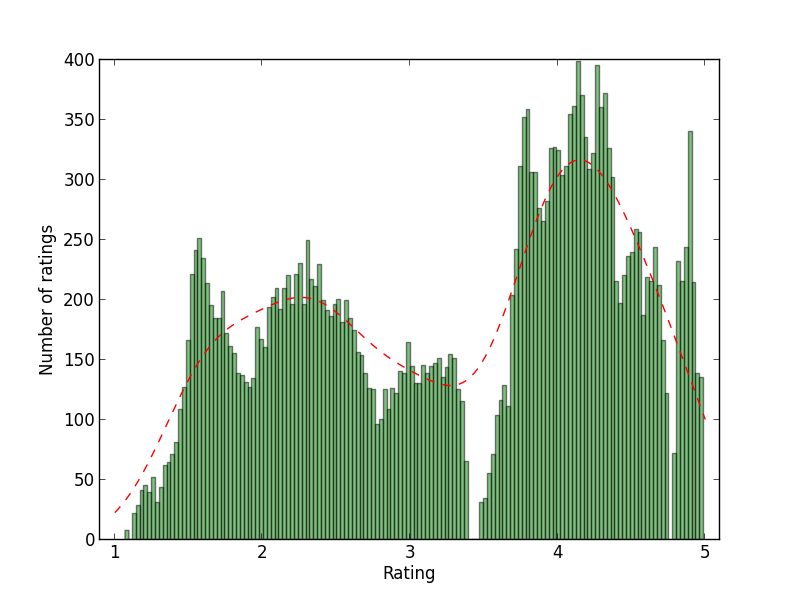
\includegraphics[scale=0.5]{image/dist-blend}
  \caption[Distribution using blend of ordering and number of days since event]{Distribution using blend of ordering and number of days since event,
  with logistic and linear penalization functions, overlayed with density
  function}
  \label{dist-blend}
\end{figure}

Especially noticeable in this distribution is that we've achieved a even
distribution without too many fluctuation. In addition there is a rounded peak
around the rating 4, which by looking at other public datasets such as in the
Netflix Prize~\cite{Netflix} or Million Song Dataset~\cite{Bertin-Mahieux2011}
is a common peak found in explicit environments. Indeed, there is a small gap
where the scores between our two events \textit{click} and \textit{want} are
bordering, a result of our sigmoid functions having a ratio of $3.5$ which
yields a gradual slope - hence when we have x-values close to $M_u$ and $0$ we
approximate $1$ and $0$ respectively, but we do not reach it exactly. This can
be seen on Figure~\ref{fig:sigmoid-penalizations}

\subsubsection{Combining recentness, popularity and price}

Instead of only looking at recentness, we can combine it with our other
features found in the previous section - namely price and popularity, as well.
As we saw by Figure~\ref{fig:dist-price} and Figure~\ref{fig:dist-popularity}, the
distribution of ratings considering both prices and popularities respectively
have peaks at edge values $1$ and $5$. When combined an item with high rating
in regards to price, but low rating considering popularity will be lowered to a
rating around $3$ - and if features are chosen coherent to what we expect the
data to represent, we expect to see a final blend where most ratings are
allocated a value around $3-4$ with few or none gaps.

\begin{figure}[H]
  \centering
  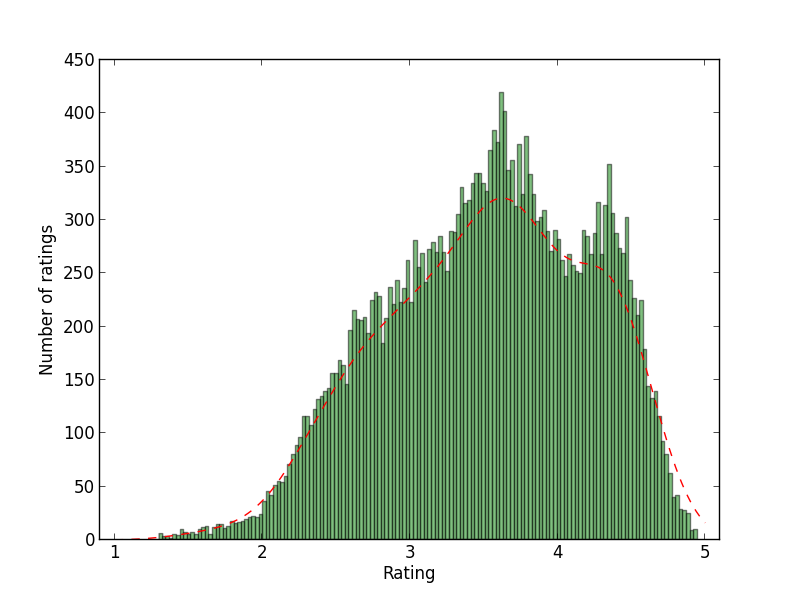
\includegraphics[scale=0.5]{image/dist-blend-price-popularity-recentness}
  \caption[Distribution using blend of price, popularity and recentness with
  linear penalization]{Distribution using blend of price, popularity and recentness with
  linear penalization, overlayed with density function}
  \label{dist-blend-price}
\end{figure}

By here combining ratings generated by recentness (both ordering and age of
events), popularity and price we see our so far "best" distribution in terms of
non quantifiable metrics. The distribution has an average rating of $3.5305$
and median $3.5780$, indicating an even spread. In the above example we have
used logistic penalization functions with constant $3.5$ as depicted in
Figure~\ref{fig:dist-recentness-sigmoid} and~\ref{fig:dist-count-sigmoid}. Using a
linear penalization function instead yields the average value $3.5293$ and
median $3.5883$, hence no large difference. The logistic approach was however
considered superior and used in future experiments as it captures the linearity
of the data, whilst in the same time accounting for seasons and the life span
of items seen in the fashion domain.

% Perhaps tell something about experiemnts that led us to choose sigmoid >
% linear?
% Any more comments on this one?

% !TEX root = ../../report.tex

\section{Recommendation Methods}
\label{sec:rec-models}

The section will introduce the different recommendation methods included in our
experiments. We have included some simple non-personalized methods in addition
to the one-class collaborative filtering methods which will be used as baselines in
our experiment. Since we want to compare traditional methods with the one-class
collaborative methods we have chosen state-of-the-art solutions from both classes
to minimize the differences.


% Since our requires us to test multiple recommender systems to get a
%better overview of added value of including implicit factors and finally our implicit ratings.
% We have also chosen to
%include some simpler non-personalized methods to be used as baseline models to
%assess whether the current system is ready for a personalized recommendation
%system. Similarly to assess the improvement, if any, over the simple
%non-personalized methods for cold-start recommendations.  E.g. one could
%imagine to final system to leverage multiple recommendation techniques. When
%users are new to the system they are recommended the most popular items, until
%enough data is collected to start providing personalized recommendations.  This
%system could be complemented by pre-computed item similarities for
%recommendations in the context of the user \emph{examining} an item. If the
%cold-start performance of these simpler models outperform the more
%sophisticated ones included in our experiments, why not just use them? However,
%our greatest problem was to find methods which in some ways could bridge the
%broken divide between binary and non-binary recommendation systems to make our
%results valid. Our solution to this is to include those methods that are
%considered state-of-the-art from both classes in an attempt to bridge this
%highly \emph{unfortunate} weakness in our experiment.


\subsection{Extracting Content-Features}


To extract features for content-based recommendations we closely examined the content in the product database.
The product descriptions had five fields in particular that we found interesting: price, brand, title, description
and meta-description. Where the first two only contain one value while the three
latter was made up of text.
Finding inspiration from the work on Ghani et. al. \cite{ghani2002building} and more closely studying the top keywords
found in the product description we decided to extract the following features:

\begin{itemize}
\item Price: grouped into price brackets
\item Brand or storename
\item Category: e.g. dress, jacket, top, pants and boots
\item Material: e.g. cotton, wool, polyester, leather
\item Style: e.g. classic, modern, comfy, sexy
\item Color
\end{itemize}

To extract the product-type, material, style and color we analyzed the content
of the title, description and meta-description fields extracting the most used
keywords after removing the stopwords, which we combined and grouped for the
different attributes. Since descriptions and titles could be either in
Norwegian or in English we had to include the words from both languages. We
also experimented with stemming from the nltk software package in Python, but
since it did not improve our results it was not used in the final
implementation. E.g. to determine if a product-type falls under the
\emph{sweater} category we check for the following keywords: \emph{sweater,
cardigan, jumper, hoody , genser and genseren} (the two latter words being
Norwegian).  The price and the brand of an item is stored in its own field,
making it an easy task to extract. \newline

It was a pleasant surprise to find out that 5,060 out of 5,855 or 86.4\% of the
items could be found in the product database and be assigned features. The
following are our feature extraction results:

\begin{table}[H]
	\centering
	\begin{tabular}{l l}
	\toprule
	Attribute & Percentage  \\ \midrule
	Price 			& 1.000 \\
	Brand 			& 0.742 \\
	Category 		& 0.628 \\
	Material 		& 0.408 \\
	Style 			& 0.314 \\
	Color 			& 0.162 \\
	\bottomrule
	\end{tabular}
    \caption[Extracted content features]{Exteacted content features in dataset}
	\label{table:extracted-content-features}
\end{table}

Price, brand and product-type can be found for \emph{most} items, while
material style and color could only be found for a minority of the items. The
dataset is in no way ideal for content-based recommendation as it highlights on
of the main weakness of content-based methods, namely that they require rich
descriptions of items to build well informed user profiles. As mentioned in
profiles. As mentioned in \cite{meyer2012recommender} this is most often not the case in
real applications. The content-features will be used to to test our one content-boosted collaborative
filtering method, BPR-Linear \cite{Gantner2010} in addition to being used by our filterbots to
rate items based on content-features.

\subsection{One-Class Recommenders}

This subsection will describe the algorithms used on the binary datasets. One-class Collaborative
filtering methods uses only binary data of the user's interaction to generate recommendations.
In addition to the methods described a user-based collaborative filtering model will be used.

\subsubsection{Most-popular Recommender}

We developed a simple most-popular recommender that uses result dithering to \emph{randomize}
the recommendations to the users. Dithering adds \emph{noise} to the algorithm, which permutes
the results in such a way that the top few results have a high probability of remaining on the top spots,
but as one goes deeper into the results, the degree of mixing increases dramatically. It is important to
note that dithering is \emph{guaranteed} to make off-line performance worse, but is likely to make the
actual performance better as the user is not presented with the same list of recommendations every
time. We experimented with two different methods of dithering:

\begin{itemize}
\item $Score = log_2(rank+x) - runif(y, z)$
\item $Score = log_2(rank+x) - y*rexp(z)$
\end{itemize}

The $runif$ function draw samples from a uniform distribution where $y$ specifies the lower boundary
of the output interval and $z$ specifies the upper boundary. The probability density function of the
uniform distribution is $P(x) = \frac{1}{z-y}$ anywhere within the interval $[y, z]$, and zero elsewhere.
The $rexp$ function draws a random number from an exponential distribution, where $z$ specifies the
$\lambda$ value, which is set to $\frac{1}{z}$. The following figure shows the exponential probability
density function given different $\lambda$ values:

% Vertical alignment of equation and plot.
\begin{figure}[H]
\label{fig:expdist}
  \centering
  \noindent\begin{minipage}{.45\textwidth}
    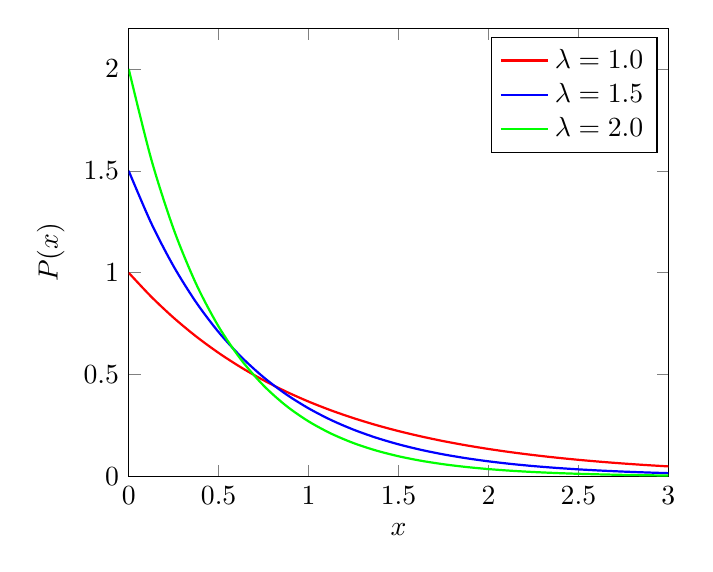
\begin{tikzpicture}
      \begin{axis}[
      	xlabel={$x$},
      	ylabel={$P(x)$},
      	ymin = 0, ymax=2.2, xmin=0, xmax=3,
      	legend entries={$\lambda=1.0$,$\lambda=1.5$,$\lambda=2.0$},
      	domain=0:3,
      ]
      \addplot[thick,smooth,red]{exp(-x)};
      \addplot[thick,smooth,blue]{1.5*exp(-1.5*x)};
      \addplot[thick,smooth,green]{2.0*exp(-2.0*x)};
      \end{axis}
    \end{tikzpicture}
    \end{minipage}
    \begin{minipage}{.45\textwidth}
      \begin{align}
        \label{exponential propability density function}
        rexp = \lambda e^{-\lambda x}
      \end{align}
      \end{minipage}
    \caption{Exponential probability density function}
\end{figure}


Given $x=5$, $y=0$ and $z=6$ using the uniform distribution dithering function we get the following
permutations in 10 runs:


\begin{table}[H]
	\centering
	\begin{tabular}{*{11}l}
	\toprule
	\multicolumn{1}{l}{\#Run} & \multicolumn{10}{l}{Result} \\ \midrule
	1 	& 8 & 3 &  24 &  20 &  1 &  19 &  22 &  15 &  42 &  36 \\
	2 	& 2 &  0 &  1 &  32 &  20 &  3 &  35 &  34 &  43 &  10 \\
	3	& 7 &  1 &  3 &  12 &  2 &  25 &  0 &  9 &  24 &  27\\
	4	& 0 &  4 &  3 &  5 &  7 &  16 &  26 &  22 &  13 &  33\\
	5	& 0 &  10 &  8 &  1 &  15 &  5 &  30 &  17 &  11 &  35\\
	6	& 7 &  4 &  6 &  12 &  2 &  1 &  19 &  0 &  27 &  9\\
	7	& 1 &  5 &  0 &  2 &  9 &  3 &  20 &  12 &  4 &  31\\
	8	& 0 &  1 &  2 &  5 &  39 &  4 &  15 &  41 &  10 &  22\\
	9	& 4 &  6 &  0 &  3 &  1 &  29 &  36 &  31 &  35 &  20\\
	10	& 5 &  1 &  0 &  8 &  3 &  18 &  25 & 24 & 2 & 28\\
	\bottomrule
\end{tabular}
\caption{Most Popular Result Dithering - Uniform Distribution}
\end{table}

The numbers specify the items original position before the ditering, e.g. item 0 was originally
the highest ranked item, item 8 was originally ranked as number 9 and so on. Given $x=1$, $y=3.0$
and $z=2.5$ using the exponential distribution we get the following permutations of the original
ranking in 10 runs:

\begin{table}[H]
	\centering
	\begin{tabular}{*{11}l}
	\toprule
	\multicolumn{1}{l}{\#Run} & \multicolumn{10}{l}{Result} \\ \midrule
	1	& 2 &  4 &  0 &  35 &  3 &  1 &  15 &  72 &  9 &  5\\
	2	& 0 &  10 &  11 &  17 &  1 &  3 &  8 &  41 &  15 &  5\\
	3	& 44 &  1 &  0 &  15 &  9 &  4 &  5 &  59 &  26 &  2\\
	4	& 0 &  98 &  1 &  4 &  2 &  41 &  8 &  26 &  11 &  94\\
	5	& 0 &  6 &  1 &  2 &  70 &  4 &  19 &  14 &  8 &  3\\
	6	& 2 &  5 &  0 &  16 &  15 &  18 &  1 &  3 &  32 &  6\\
	7	& 2 &  65 &  4 &  0 &  3 &  45 &  8 &  1 &  48 &  36\\
	8	& 3 &  49 &  5 &  0 &  2 &  82 &  8 &  77 &  11 &  4\\
	9	& 0 &  1 &  21 &  8 &  4 &  85 &  2 &  6 &  47 &  3\\
	10	& 0 &  1 &  21 &  70 &  11 &  20 &  2 & 10 & 9& 3 \\
	\bottomrule
\end{tabular}
\caption{Most-Popular Result Dithering - Exponential Distribution}
\end{table}

As you can see the lists generated are quite different. The uniform distribution has a lower occurence of higher
numbers in the lists, but it also has a smaller occurrence of smaller numbers. The exponential distribution
goes as far as including an item that originally was ranked 98th. This is due to the fact that the exponential
distribution can output large values, in theory up to infinity, with a decreasing probability.
However, you can also see that the highest ranked items is consistently found at the top of the list
for the exponential function.
To get a clearer image of their differences consider the following figure which shows the minimum, maximum and average position of
the first 10 items for 100 over recommendations using the same parameters as above:

\pgfplotstableread{
x    y    	y-max  	y-min
0 	1.40 	3.60 	1.40
1 	3.18 	6.82 	3.18
2 	5.25 	6.75 	5.25
3 	6.40 	7.60 	6.40
4 	9.28 	10.72 	9.28
5 	10.77 	13.23 	10.77
6 	11.57 	12.43 	11.57
7 	13.73 	15.27 	13.73
8 	15.42 	13.58 	15.42
9 	16.04 	13.96 	16.04
}{\expdist}

\pgfplotstableread{
x    y    	y-max  	y-min
0	3.56	15.44	3.56
1	5.91	25.09	5.91
2	8.69	22.31	8.69
3	12.31	34.69	12.31
4	12.69	40.31	12.69
5	15.74	36.26	15.74
6	19.99	42.01	19.99
7	21.05	41.95	20.05
8	24.73	42.27	23.73
9	23.71	45.29	23.71
}{\uniformdist}

\begin{figure}[H]
	\label{fig:minmaxuniform}
	\centering
	\begin{tikzpicture}
	\begin{axis} [
		ymin=-5,
		xlabel={Original Position},
		ylabel={Position After Dithering},
	    symbolic x coords={0,1,2,3,4,5,6,7,8,9},
	    xtick=data
	]
	\addplot [only marks, red]
	  plot [error bars/.cd, y dir=both, y explicit, error bar style={line width=2pt}]
	  table [y error plus=y-max, y error minus=y-min] {\uniformdist};
	\addplot [only marks, blue]
	  plot [error bars/.cd, y dir=both, y explicit]
	  table [y error plus=y-max, y error minus=y-min] {\expdist};
	\end{axis}
	\end{tikzpicture}
	\caption[Average position of recommendations with dithering]{Minimum, maximum and average position of 10 first items over 100 recommendations for the exponential distribution dithering (blue) and uniform distribution dithering (red)}

\end{figure}

The figure show that the exponential distribution varies the position of the first items much less
than the uniform distribution, never putting the highest ranked item lower than number five in the
list while the uniform distribution puts it as far back as 20th. The values of $x$, $y$ and $z$ can be modified to
achieve the desired degree of mixing.

\subsubsection{One-Class Item-based Collaborative Filtering}

There are a number of different ways to compute the similarities between items given binary preference data.
Here we present one such method called \emph{log likelihood}, which is implemented in Mahout \cite{mahout}
Log Likelihood Similarity is used to score and analyze counts of events, particularly counts of when events occur together.
The counts you have in these situations are the following:

\begin{itemize}
\item $c_{11}$ the number of times two events have occurred together
\item $c_{12}$ and $c_{21}$ the number of times one occurred without the other.
\item $c_{22}$ the number of times something was observed that was neither.
\end{itemize}

Once you have these counts the log likelihood $G^2$ can be computed as follows:\newline

\begin{subequations}
$G^2$ = 2(matrixEntropy(c)-rowEntropy(c)-columnEntropy(c))
\begin{align}
	rowEntropy(c) = H(c_{11}, c_{12}) + H(c_{21}, c_{22}), \\
	colEntropy(c) = H(c_{11}, c_{21}) + H(c_{12}, c_{22}), \\
	matrixEntropy(c) = H(c_{11}, c_{12}, c_{21}, c{22}),
\end{align}
\end{subequations}

where $H$ is Shannon's entropy, which can be computed using the following formula:

\begin{equation}
H(X) = - \sum_{i} x_i log \frac{x_i}{N} = -N \sum_i \frac{x_i}{N} log \frac{x_i}{N}
\end{equation}

where $N$ equals $\sum_i x_i$. Using the above notation Shannon's entropy for $H(c_{11}, c_{21})$ gives us:

\begin{equation}
H = (c_{11} + c_{12})log(c_{11} + c_{12})-c_{11} log(c_{11}) - c_{12} log(c_{12})
\end{equation}

In addition to log likelihood we will also experiment with the cosine similarity model
found in MyMediaLite \cite{Gantner2011MyMediaLite}.

\subsubsection{BPR: Bayesian Personalized Ranking}

BPR presented by Rendle et. al. \cite{Rendle2009} can be used to learn the latent factors of a
latent factor model using binary implicit feedback. For our experiment we have used to implementation
found in MyMediaLite \cite{Gantner2011MyMediaLite}. Bayesian Personalized Ranking was designed for the item
prediction task and optimized for ranking using implicit feedback such as e.g. purchases in an online shop.
The task of the recommender system is to provide the user with a personalized ranking $>_c \subset I^2$ of all
items, where $>_c$ has to meet the properties of a total order. Finding the personalized ranking for all items
$s \epsilon S$ is to maximize the following posterior probability where $\theta$ represents the parameter vector
of an arbitrary model in our case a matrix factorization model.

\begin{equation}
p(\theta | >_c) \propto p(>_c | \theta) p(\theta)
\end{equation}

Where $>_c$ is the desired but latent preference structure for user $c$. All users are presumed to act
independently of each other. The ordering of each pair of items is assumed to independent of every other pair.
The generic optimization criterion for personalized ranking is as follows:

\begin{equation}
BPR(D_S) = \underset{\theta}{\arg\max} \sum_{(c,i,j)\epsilon D_s} ln \sigma(\hat{u}_{c,i}(\theta)-\hat{u}_{c,j}(\theta)) - \lambda \left\|\theta \right\|
\end{equation}

Here $D_s$ is the binary dataset used, $\sigma(x)$ is the logistic sigmoid function, $\theta$ represents
the model parameters, $\hat{u}_{c,s}$ is the predicted score for user $c$ and item $s$ and
$\lambda \left\|\theta \right\|$ is the regularization term. It reduces the model learning task to
a pairwise classification problem.\newline

BPR learns the model parameters $\theta$ as follows using stochastic gradient descent:

\begin{itemize}
\item Step 1: Draw (c,i,j) from $D_S$
\item Step 2: $\theta \leftarrow \theta + \alpha \left\lgroup \frac{\exp^{-\hat{x}_{cij}}}{1+\exp{\hat{x}_{cij}}}  \frac{d}{d \theta} \hat{x}_{cij} + \lambda_{\theta} \theta \right\rgroup$
\item Step 3: Repeat step 1 and 2 until convergence
\end{itemize}

where $\alpha$ is the learning rate and $\lambda_{\theta}$ is the regularization constant. BPR will hereby be
referred to as BPR-MF.

\subsection{Non-Binary Recommenders}

The following recommenders will be used to test our implicit ratings. In addition to the methods described,
traditional user-based and item-based collaborative filtering described in Section~\ref{subsubsec:memory-based} will
also be used.

\subsubsection{ALS-WR}

%Implicit Feedback Recommendation via Implicit-to-Explicit Ordinal Logistic Regression Mapping

ALS-WR is the only method which we have found that \emph{supports} implicit ratings, making
it a natural part of our experiment. For our experiment we have used the Mahout \cite{mahout} implementation.

Alternating-least-squares with weighted-$\lambda$-regularization (ALS-WR) was designed fro the Netflix Prize
Competition \cite{Netflix}, where it obtained an RMSE score of 0.8975, which was one of the best results based
on a pure method. As you may know, the Netflix Prize Competition was won using an ensemble of multiple predictors.

Alternating-least-squares is a method to solve Equation~\ref{equation:minimize}. Since both $q_{s}$ and $p_{c}$
are unknown, the equation is not convex. However if we fix one of the unknowns, the optimization problem becomes
quadratic and can be solved optimally. The ALS technique rotate between fixing the $q_{s}$'s and fixing the $p_{c}$'s.
When all the $p_{c}$'s are fixed, the system recomputes the $q_{s}$'s by solving a least-squares problem, and vica versa.
This ensures that each step decreases the error until convergence. What makes ALS favorable over the simpler and faster
stochastic gradient descent is two things. ALS can be parallelized since the system computes the $q_{s}$'s independently
of the other item factors, the same can also be applied to the user factors. The second case if for systems centered around
implicit data. Because the training set cannot be considered sparse, looping over each single training case as gradient descent
would not be practical, but ALS can efficiently handle such cases \cite{Hu2008}.\newline

ALS solves the low-rank matrix factorization as follows:

\begin{itemize}
\item Step 1: Initialize the matrix M by assigning the average rating for that movie as the first row, and a small random numbers for the remaining entries;
\item Step 2: Fix P, solve Q by minimizing the objective function (the sum of squared errors);
\item Step 3: Fix Q, solve by minimizing the objective function similarly;
\item Step 4: Repeat Steps 2 and 3 until a stopping criterion is satisfied.
\end{itemize}

Without regularization ALS might lead to overfitting due to the many free parameters. Regularization was
therefore introduced in the form of weighted-$\lambda$-regularization to prevent the model from overfitting.

\begin{equation}
f(P, Q) = \sum_{(c,s)\epsilon C} (u(c,s) - p^{T}_{c}q_{s})^{2} + \lambda (\sum_{c} n_{p_{c}} \Vert p_{c} \Vert ^{2} + \sum_{s} n_{q_{s}} \Vert q_{s} \Vert ^{2})
\label{WeightedLamba}
\end{equation}

where $n_{p_{c}}$ and $n_{q_{s}}$ denote the number of ratings of user $c$ and item $s$ respectively. $S_{c}$ denote
the set of items $s$ that user $c$ rated, then $n_{p_{c}}$ is the cardinality of $S_{c}$; similarly $C_{s}$ denotes
the set of users who rated item $s$, and $n_{q_{s}}$ is the cardinality of $I_{s}$. A given column of P, $p_{c}$ is
found by solving a regularized linear least squares problem involving the known ratings of user $c$, and the
feature vectors $q_{s}$ of the items that user $c$ has rated. Similarly, we can compute individual $q_{s}$'s via
a regularized linear least squares solution, using the feature vectors of users who rated item $j$, and their ratings of it.
The implicit feedback extension of the method is described in~\ref{implicit-als-wr}.

\subsubsection{Item-Average}

Item average is a simple recommender that always estimates the preference for an item to be the average of
all known preference values for that item. No information about the individual users is taken into account.
This recommender can therefore be considered a \emph{highest rated} recommender, as it is likely to recommend
the highest rated items. The following equation shows the rating prediction procedure:

\begin{equation}
\label{equation:itemaverageratingprediction}
u(c,s) = k * \sum_{c' \epsilon C} u(c',s)
\end{equation}

where $k$ is a normalization factor ($1/|C|$). This is very similar to collaborative filtering, except for
the fact that the user similarity $sim(c, c')$ has been taken out of the equation. This is the same as saying
that all user similarities are the same. It is also worth mentioning that this method is not suited for binary
ratings, is it need ratings to average on.

\subsection{Cold-start Solution}

Due to limitations, mainly in the form of a lack of additional data sources the cold-start solutions
we are currently able to experiment with is fairly limited. As we never got access to
user-data, we have to cross out RBLF and other methods requiring user features. This leaves us with
Naive Filterbots \cite{Park2006} which easily could be combined with our implicit ratings.

\subsubsection{Filterbots}
\label{implementation-filterbots}

The main reasons for experimenting with filterbots is simplicity, the fact that it easily could
be combined with our implicit ratings in addition to the fact that previous experiments \cite{Agarwal2009, Agarwal2010}
show that its performance is close to the state-of-the-art methods. It is worth to keep in mind that filterbots was
developed for traditional neighborhood collaborative filtering methods, and will therefore only be applicable given
that a neighborhood model is chosen as the core recommender. Filterbots can potentially help solve the cold-start user
problem by making it possible for new users to connect to pseudo users that capture the general underlying trends of the entire
user group. Filterbots were designed to improve performance when data is scare without degrading performance when the data
is plentiful.

Similarly as in \cite{Park2006} we decided to experiment with \emph{naive} global bots. The bots are \emph{naive}
in the sense that they are \emph{dumb} in the way they rate items, e.g. by only considering one item-attribute of the items.

We have currently implemented the following bots:

\begin{itemize}
\item BrandBot: rates all items based on the average brand rating
\item SingleBrandBots: multiple bots that give all items of a specific brand a maximum rating
\item PopularityBot: rates all items based on their popularity
\item AverageBot: rates all items based on their average rating
\item CriticBot: $n$ critics among the most active users are selected and rate items based on the average
	  rating given by these critics.
\end{itemize}

The \emph{PopularityBot} estimates each rating using the following formula: $r(c,s) = log_{3}C_{s}$, where $C_{s}$ is the number of users which have rated the item and $3$ is a normalization constant that caps the ratings a little below 5, which is our maximum rating.
Compared to the work presented by Park et. al. we felt that the lack of high quality features was a limiting factor when designing the filterbots, as most features would not let us rate most ratings, and there is only so much information in the rating matrix.

The intuition behind the \emph{SingleBrandBots} is as follows, given that a user-based collaborative filtering algorithm is used:
when a new user \emph{rates} an item of a single brand it will be connected with one such bot. The user can then be recommended
items from this bot's list, meaning that the user can be recommended items of the same brand. Which in theory, should be better
than recommending some item from a random brand. Similarly, the \emph{PopularityBot}
will have rated the popular items highly meaning that new users that connect to this psuedo user will be recommended the
most popular items. For item-based methods it works a little differently as it only has an effect on the item-similarity matrix.
Since more item similarities can be defined due to the psuedo users, more neighbors for the target item can be chosen from the candidate set.

Both the \emph{AverageBot} and \emph{BrandBot} can be seen to incorporate the implicit rating factors such as recency into
the ratings generated. However, for the \emph{PopularityBot} and \emph{CriticBot} we wish to implement additional functionality to ensure
that the new users are connected with items that are relevant right now and not consider outdated items or users which
are no longer active. Since we have access to timestamps we could e.g. make the \emph{PopularityBot} rate items based on
their popularity the last couple of weeks instead of over the entire dataset period. Similarly, critics can be selected
based on their activity the couple of weeks/months.

\subsection{Test Suite}

As many of our selected evaluation metrics not is implemented in the recommender system libraries used we implement our own test suite. It is a bash
script that takes the entire log file as input first transforming it to into a set of ratings, or blend of your choice before splitting it based on timestamps
or simply generating a random split. These outputs are then fed into either Mahout or/and MyMediaLite training the specified models and writing their predictions to file. Our evaluation suite then calculates all the metrics desired writing them out in a latex format. All in one command line call. Our evaluation suite currently supports nDCG, $MAP@K$, User and Item-Space Coverage, hLU, MPR, in addition to our own unique simple event evaluator. The current functionality is
highlighted in the listing below:

\begin{lstlisting}
$ ./testsuite.sh -h
Usage: ./testsuite.sh [options]

This program can do the following depending on the options provided:
  - Generate a set of implicit ratings based on an event log.
  - Recommend based on methods provided either by Mahout or MyMediaLite.
  - Evaluate the results yielding MAP@20, AUC and ROC.
  - Write the result to a latex-table, for easy exporting to a report.

OPTIONS:
  -a <filterbot settings> A string defining which filterbots to enable.
                          Defaults to '0,0,0,0,0'.
  -c                      Clean existing rating, prediction and scoring files
                          before running.
  -i <input file>         The absolute path to the event log file.
  -f <product features>   The absolute path to file containing all product
                          features obtained from the product DB.
  -d <product file>       Where to find product file with JSON-data, used with
                          cold-start splits. Defaults to 'generated/products.txt'
  -r <rank recommenders>  Which rank recommenders to user with MyMediaLite.
  -p <item recommenders>  Which item recommenders to use with MyMediaLite.
  -m <mahout algorithms>  Which recommender algorithms to use with mahout.
  -s <split type>         How to split test and training. Options: 'cold',
                          'time' or 'random'.
  -k <k values>           When using ItemKNN, control which k-values to use, as
                          a string of integers. E.g. '10 20 50'
  -b                      Convert all ratings to binary (all ratings to 1)
  -q                      Send stdout and stderr to /dev/null (except result)
  -t                      Split coldstart on time
  -l                      Run recommender on blend file only.
  -h                      Display this help-information.

RANK RECOMMENDERS:
  The following algorithms are available to use with the rank recommender
  provided by MyMediaLite:
    BiPolarSlopeOne, GlobalAverage, ItemAttributeKNN, ItemAverage, ItemKNN
    MatrixFactorization, SlopeOne, UserAttributeKNN, UserAverage
    UserItemBaseline, UserKNN, TimeAwareBaseline
    TimeAwareBaselineWithFrequencies, CoClustering, Random, Constant
    LatentFeatureLogLinearModel, BiasedMatrixFactorization, SVDPlusPlus
    SigmoidSVDPlusPlus, SocialMF, SigmoidItemAsymmetricFactorModel
    SigmoidUserAsymmetricFactorModel, SigmoidCombinedAsymmetricFactorModel
    NaiveBayes, ExternalRatingPredictor, GSVDPlusPlus

ITEM RECOMMENDERS:
  The following algorithms are available to use with the item recommender
  provided by MyMediaLite:
    BPRMF, ItemAttributeKNN, ItemKNN, MostPopular, Random
    UserAttributeKNN, UserKNN, WRMF, Zero, MultiCoreBPRMF
    SoftMarginRankingMF, WeightedBPRMF, BPRLinear, MostPopularByAttributes
    BPRSLIM, LeastSquareSLIM

MAHOUT RECOMMENDERS:
  The following methods are available when using Mahout:
    svd, itembased, userbased, itemuseraverage, loglikelihood, itemaverage

Examples:
  Split randomly and calculate the itemaverage with mahout:
  ./testsuite.sh -i ../somefile.tab -s random -m 'itemaverage'

  Split on time and use itemKNN with various K-values to do recommendations:
  ./testsuite.sh -i ../somefile.tab -s time -p 'ItemKNN' -k '10 20 50'

  Split with cold start and use some filterbots:
  ./testsuite.sh -i ../somefile.tab -s cold -m 'userbased' -a '1,1,1,0,0'
\end{lstlisting}

% !TEX root = ../../report.tex
\clearpage
\section{Experimental Plan}
\label{sec:experimental-plan}

%We can sometimes evaluate how well the recommender achieves its overall goals.
%For example, we can check an e-commerce website revenue with and without the
%recommender system and thereby estimate the value of the system to the website.

In this section we present our plan to validate our methods. We first introduce
the main goals for our experiment, then discuss how we plan to achieve them.
The second part therefore touches on our evaluation methodology.
We have the following main goals for our experiment:

\begin{itemize}
	\item Goal 1: determine the effect of utilizing multiple event types
	\item Goal 2: determine whether our proposed implicit rating methods improve the recommendation quality over
		  		  using \emph{more simplistic} binary methods.
	\item Goal 3: evaluate the different implicit factors and attempt to quantify their importance.
	\item Goal 4: quantify if our cold-start solution adds any value to the system.
\end{itemize}

\subsection{Experimental Datasets}

As previously mentioned the SoBazaar dataset is both small and sparse.
Having such a small and sparse dataset has several implications. Firstly we have
to avoid \emph{wishful thinking} as we have very thin data, meaning that we cannot
rely on getting reliable results. Secondly, our evaluation methodology must be
\emph{tailored} for small sparse datasets. E.g. when using cross-validation the number
of folds depends on the size of the dataset. For large datasets, even 3-fold Cross
validation will be quite accurate, while for very sparse datasets, one may have to
use leave-one-out in order to train on as many examples as possible. The advantages
of using a large number of folds is that the bias of the true error rate estimators
will be small, meaning that the estimator will be very accurate, with the disadvantages
being that the variance of the true error rate estimator will be large in addition to
increased computation time. Another alternative well suited for sparse datasets is the
\emph{all but one} or the \emph{leave one out} method, in which we remove one rating
from the test users and try to predict the hidden rating.
Another important concern is whether or not to take the timestamps into consideration,
which directly speaks against the use of cross-validation, as we wish to use the past
interactions to predict future actions. When using the \emph{leave one out} method one
could always remove the users freshest rating and try to predict it and repeat the
process any number of times. This is particularly relevant as some of our implicit
mapping functions factors in recency.

We chose to utilize both time-splits and random splits to improve our confidence
in our results. For both splits we repeat the process 10 times to get as reliable
estimates as possible. The following table shows an overview of the experimental datasets.

\begin{table}[H]
    \centering
    \begin{tabular}{l l l l l l }
    \toprule
	Dataset						& 	Ratings		& 	Users		& 	Items 		& 	Sparsity	& Rating Scale 				    \\ \midrule
	Sobazar	(Purchases Only) 	&	1,592		&	466			&	1188		&	99.71243	& Binary						\\
	Sobazar (All events)		& 	27,873  	& 	1,532		&	5688		& 	99.69657	& Binary/Implicit Ratings		\\
	\bottomrule
    \end{tabular}
    \caption [Experimental datasets]{General overview of the datasets used for evaluation}
    \label{table:datasets}
\end{table}

As you can see the recommender can cover a much larger portion of the user group
and items when including multiple event types. However, the sparsity is only reduced slightly
as the number of items and users are much higher.


\subsection{Evaluation Methodology}

The following paragraphs will describe our methodology for testing and verifying our experimental
goals.

\paragraph{Goal 1}

We want to measure if there is any added value to using multiple implicit factors compared to
looking at purchase data only. Meaning that we want to measure whether a recommender that utilizes
data including multiple implicit factors improve the recommendation quality. This can not
easily be measured using traditional measures due to the fact that the datasets contains
different users and items. In addition to measure their quality, by means of different
evaluation metrics, one must also make a few assumptions regarding the importance
of the different events. Our main assumptions are that it is better to recommend a clicked
item than a random item, and that the same also applies to wants. This means that our comparison
will be made on a somewhat subjective basis. The additional coverage will also be factored in. 

\paragraph{Goal 2}

We want a way to measure if our proposed models outperform the \emph{simpler} one-class
collaborative filtering methods. The main problem with this is that our main contribution
are the ratings that are fed into the recommender, and that we are forced to use different
methods for providing recommendation. Optimally, we would like every variable to be fixed
to get the most reliable results. In an attempt to \emph{mitigate} this problem, we 
have carefully selected methods which we consider to be the state-of-the-art from both segments
to make the comparison as fair as possible. The comparison of recommendation quality
is mainly a evaluation metric problem and will be discussed at greater length in
Section \ref{sec:eval-metrics}.

\paragraph{Goal 3}

We want to learn which implicit factors are the most \emph{important} with regard to
improved recommendation quality. Our success then relies on that we successfully can compare
a set of ratings, which is something you not often encounter in the literature. As we currently
are limited to offline studies we have to make a few assumptions to perform the comparison.
Our main assumption is that better ratings will produce better recommendation results,
which we believe to be a fair assumption, as ALS-WR especially is designed to take
in ratings with different confidence levels attached to them. Thus, making this
problem mainly an evaluation metric problem, which is discussed at greater
length in Section \ref{sec:eval-metrics}. This allows us to input different sets
of ratings generated incorporating different implicit factors and see which implicit
factors improve our results the most.

\subsection{Goal 4}

We wish to learn whether or not our filterbots enhance our systems ability to handle
the three different cold-start related problems. This means that we need some methodology
to be able to simulate the different cold-start scenarios and measure the recommendation quality.
As mentioned in Section~\ref{sec:cold-start-eval} there is no common framework for assessing 
the cold-start performance of recommender systems. To recap the cold-start problem and how
the dataset changes over time we have three main input types:

\begin{itemize}
	\item 	Existing users watch new items in the catalogue
	\item	New users join the system and view their first item
	\item	New items are added to the catalogue
\end{itemize}

The first input source has the effect of increasing the dataset density, while
the latter two has the opposite effect. To simulate a new user entering the system
we adopt a methodology similar to the one described in \cite{Stern2009, Lam2008}. The
users are split in two disjoint sets, setting aside 10\% of the users as test users.
We introduce a selection criteria similarly to the one described in \cite{Rashid2002, Rashid2008}
where we only select users that have given above 20 ratings as eligible test users,
then selecting a random subset of these users.
We then train three different models using 10\%, 40\% and 75\% of the test users
ratings and try to predict their remaining ratings. The same methodolgy is applied
to test items, the only difference being that only 5\% of the items are used as 
test items due to a low number of average ratings per item. The selection criteria
for items is set to a minimum of 15 ratings.

To evaluate the cold-start system performance we use the same method as
described in ~\cite{Agarwal2009}. We use a 80:20 split where the same 20\% is set
aside for testing. We then randomly draw 40\%, 60\% and finally 80\% (all) ratings
and see how well our method perform for the different sparsity levels.
It is important to note that this process should be repeated multiple times, as
the chance of getting an \emph{unfortunate} split is highly probable due to the
dataset size.

We perform both random and time-based splits. For our time based
splits we train the model with ratings in chronological order, e.g. using
the 10\% of the first ratings for a user, where his later activity is put in the testset.
Similarly for the cold-start system splits we train the model using different random subset
of the 80\% earliest ratings and try to predict the remaining 20\%.

\subsection{Generalization Properties}

We were unable to acquire any e-commerce datasets containing user browsing history including different
event types and timestamps. Although we inquired other researchers having experimented with similar
datasets to no luck.

In addition to evaluate the methods on the SoBazaar dataset wanted to verify that our
methods generalizes beyond our experimental dataset, in accordance to the general guidelines
for experimental studies \cite{Shani2011}. The data used for offline evaluation should match
as closely as possible the data we expect the recommender system to face when it is
deployed \cite{Gunawardana2009}. When searching for datasets for evaluation we focused on the
following dataset properties:

\begin{itemize}
	\item Size of dataset: Preferable as close as possible to SoBazaar or larger (a few months from now)
	in terms of number of ratings, users and items.
	\item Different different types of implicit factors	such as clicks, likes and purchases.
	\item Domain: Preferably a domain as close to possible as the e-commerce domain where
	factors like recency also would apply.
	\item Timestamps: To evaluate the recentness mapping
	\item Presence of features (Secondary)
\end{itemize}






% !TEX root = ../../report.tex
\section{Evaluation Metrics}
\label{sec:eval-metrics}

%http://www.slideshare.net/gunnar-schroeder

This section will discuss the suitedness of different evaluation metrics in the context
of measuring the recommendation quality for SoBazaar and \emph{G8} of our thesis.

\textbf{G8} automatically disqualifies metrics that consider the ratings themselves as the
ground truth and bases its evaluation score on these numbers. MAE and RMSE can therefore
confidently be crossed off the list of suited metrics.

As for Sobazaar, the main reasons for implementing a recommender system is the desire to improve user
satisfaction and to increase the economic success of a platform. In order to further specify what
defines \emph{good recommendation quality} for SoBazaar, we have to take a closer look at the
recommender's task, the application interface and the data available. The following figures
shows the SoBazaar newsfeed and how the personalized recommendations are to be shown to the user:

\begin{figure}[H]
		\begin{subfigure}[b]{.45\linewidth}
			\centering
	  	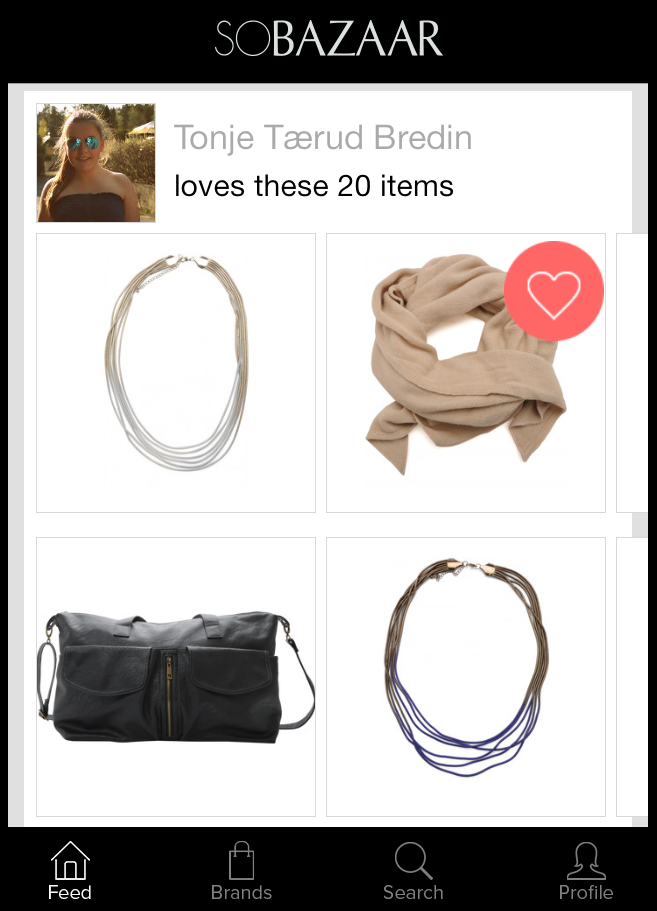
\includegraphics[scale=0.25]{image/SoBazaarfeed2.png}
		\end{subfigure}
		\begin{subfigure}[b]{.45\linewidth}
			\centering
			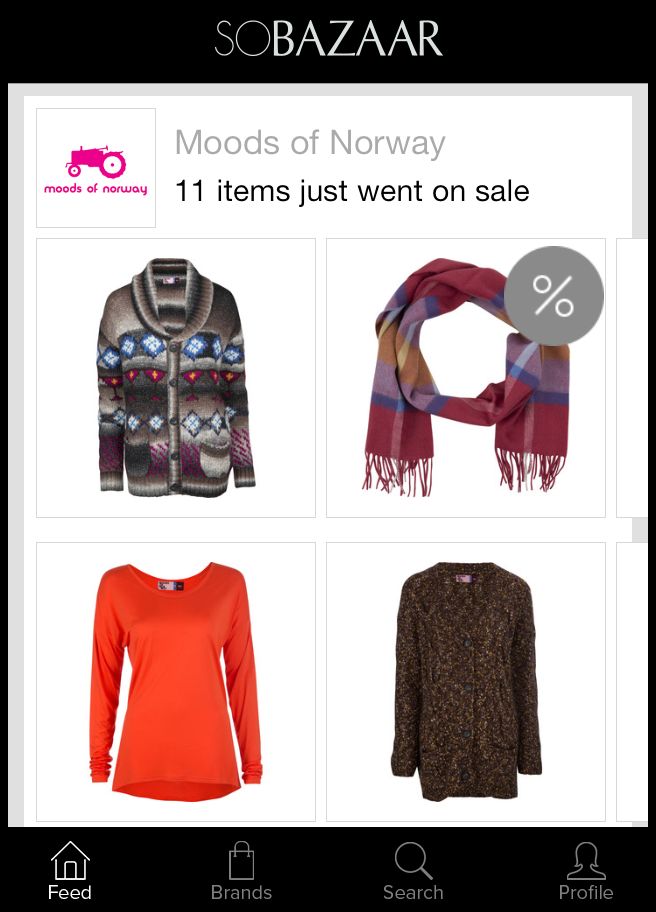
\includegraphics[scale=0.25]{image/SoBazaarsale.png}
		\end{subfigure}
		\caption[Sobazaar News Feed - Version 0.5.1]{SobBazaar news feed items}
		\label{figure:sobazarfeed}
\end{figure}

The most typical task for a e-commerce recommender system is to determine an order of item, often with the
purpose of creating a top-K list of recommendations that is shown in a sidebar or on a dedicated page.
In the case of SoBazaar they are shown in a feed item, showing up to 20 items, making a K value of 20
a natural choice. This makes it safe to assume that the users are more interested in the to ranked items,
than rating predictions for  the entire item collection. Evaluation of top-20 recommendations therefore
suggest a classification or ranking task. An accuracy metric will tell us something the recommenders
ability of retrieving relevant items while a ranking accuracy metric should measure how well the different
methods are at ordering or ranking these predictions. The fact that only 4 recommendations are initially shown,
requiring the user to scroll to view the remaining items highlights the importance of measuring the ranking quality.
We also assume that some items are more relevant than others, e.g. that metric should reward
the recommender for constantly ranking purchases over less relevant events such as clicks.

\subsection{Accuracy Metrics}

Due to the fact that we are working with a highly sparse dataset with a large item collection
it is reasonable to believe the the likeliness of finding a hidden item in the top-20 recommended items
is not very high. We therefore felt that The Area Under Curve (AUC), described in Section \ref{sec:relevance-based}
would be a nice complement to the rank accuracy metrics. AUC allows us to measure the recommenders overall
ability to retrieve relevant items and can therefore be used as a single measure for the overall quality of a recommender
system. Not only considering the top results.

One should be aware of that the AUC scores can be highly inaccurate, especially for cold-start users,
users which the recommender is unable to provide more than a handful of recommendations for. AUC requires
a total ordering of all items not yet rated by the user. This means that the items not recommendable
to the user will be appended in a random order after the known recommendations.
E.g. lets say the recommender is able to generate 10 recommendations for a user out of 4000 items.
The recommender was only able to retrieve one out of two relevant test items. The remaining 3990
items are therefor appended in random order to the users recommendation list. Where the last test item is
appended in the recommendation list can mean the difference between a AUC score of above
0.9 to less than 0.6 if the item is appended at the end of the list, the results can be even more
severe if none of the items is in the initial recommended list, then the results for that user will be
completely random. The most obvious solution to this problem would be to use resampling or to repeat
the experiment multiple times where the order of the items not in the recommendation list are drawn at random and
the results averaged over all the trials.

A frequently uttered point of criticism is that users are often more interested in the items
at the top of a recommendation list but that the AUC measure is equally affected by swaps at the top
or the bottom. Which explains why AUC is not sufficient alone in our case.

\subsection{Rank accuracy}

The introduction gave us two clues that should be considered when selecting a rank accuracy metric.
(1) a ranking accuracy metric that measures the overall ranking is not appropriate, (2) the ranking
metric should be able to account for the different relevance levels.
Again, we assume that we can recommend at most $20$ items for each user at a time. It also pays to submit all $20$
recommendations, because we are not penalized for bad guesses. We also assume that the order matters, so it
is better to submit more certain recommendations first, followed by recommendations we are less sure about.
Which means that we basically select the $20$ best candidates in order. 

<<<<<<< HEAD
Mean average precision $MAP@k$, described in Section~\ref{subp:mean_average_precision_map_} is a popular metric for search
engines and is applied, for example, to report results at the Text Retrieval Conference (TREC). $MAP@20$ will give us a score
of how many items we are able to retrieve and how high up in the recommendation list they are placed. The main weakness in our
case is that it assumes all items to be equally relevant, meaning that it has no way of factoring in the different event types.

Normalized Discounted Cumulative Gain (nDCG) described in Section \ref{subp:normalized_discounted_cumulative_gain_} is a popular metric for
measuring the rank accuracy. It is based on two main assumptions; (1) Highly relevant items are more useful than marginally relevant ones,
=======
Mean average precision (MAP@k), described in Section~\ref{subsec:offlineeval} is a popular metric for search
engines and is applied, for example, to report results at the Text Retrieval Conference (TREC). The main weakness with regard
to recommender systems is that it assumes that the user is interested in finding many relevant documents for each query, and
does not look at the relevance of the items. Consider the following examples where we have three lists of hidden items and
three recommendations lists. All none relevant items are labeled with the item-id $0$.

\begin{table}[H]
\label{table:ap}
\centering
\begin{tabular}{*{4}l}
\toprule
Example 	& 	Actual					& 	Recommended					&	AP@10   \\ \midrule
1			& [1,2,3,4,5,6,7,8,9,10]	&	[1,0,0,0,0,0,0,0,0,0]		&	0.100  \\
2			& [1,2,3,4,5,6,7,8,9,10]	&	[1,0,0,0,2,0,0,0,0,0]		&	0.140  \\
3			& [1,2,3,4,5,6,7,8,9,10]	&	[8,0,0,0,9,0,0,0,0,0]		&	0.140  \\
4			& [1,2,3,4,5,6,7,8,9,10]	&	[1,0,0,0,3,0,5,0,0,0]		&	0.183  \\
5			& [1,2,3,4,5,6,7,8,9,10]	&	[0,0,0,2,0,0,0,6,5,0]		&	0.083  \\
6			& [1,2,3,4,5,6,7,8,9,10]	&	[0,0,0,0,7,0,8,0,0,0]		&	0.049  \\
7			& [1,2,3,4,5,6,7,8,9,10]	&	[0,0,0,0,7,0,0,0,0,1]		&	0.040  \\
8			& [1,2,3,4,5,6,7,8,9,10]	&	[0,0,0,0,0,0,0,8,5,0]		&	0.035  \\
9			& [1,2,3,4,5,6,7,8,9,10]	&	[1,3,4,5,6,0,0,0,0,0]		&	0.500  \\
10			& [1,2,3,4,5,6,7,8,9,10]	&	[0,0,0,0,0,1,2,8,5,3]		&	0.178  \\
\bottomrule
\end{tabular}
\caption{$AP@10$ Examples}
\end{table}

As you see from example two and three average precision does not consider the order of the actual item list. We want some way to
reward the recommender for getting the purchased ranked higher than both wants and clicks.

Normalized Discounted Cumulative Gain (nDCG) described in Section~\ref{subsec:offlineeval} is another metric to
measure the rank accuracy. It is based on two main assumptions; (1) Highly relevant items are more useful than marginally relevant ones,
>>>>>>> f0332291a5f01c7cee3f7a798995f919497c3c5c
(2) The lower the ranked position of a relevant item, the less useful it is for the user, since it is less likely to be \emph{examined}.
The maybe most interesting aspect of nDCG is that it contains an utility function $rel_i$. One can replace the original utility function
and replace it with a function that is more suited to the application. One could e.g. assign the relevance of an item using
the following functions:

\begin{itemize}
\item $rel_i = 1/log(i+k)$: where $i$ is the index of the item in the actual sorted rating list, where $k$ is a constant.
\item $rel_i = u(i)$: simply assign a relevance or utility score such as e.g. the rating of the item or the event type score.
\end{itemize}

The latter would have been perfect, given that we could specify the importance of each event e.g. purchase gets a relevance of 3, want
a relevance of 2 and a click a relevance of 1, as it would give us a single number on the ranking quality of the recommendations.
However, we do not not know these values, meaning that nDCG cannot be used without making assumptions about the importance of the different
event types. To solve this problem we decided to chose a \emph{simpler} approach. We independently measure the recall
and counts of clicks, wants and purchases retrieved by the recommender in the top 20 positions. As you see, it would have been nice to know these
<<<<<<< HEAD
reward attributes to make the evaluation results more \emph{reader friendly}. To check if an user-item touple is a click, want or purchase we create
a file which stores the log events in the following format:
=======
reward attributes to make the evaluation results more fluent.

To check if an user-item tuple is a click, want or purchase we create a file which
stores the log events in the following format:
>>>>>>> f0332291a5f01c7cee3f7a798995f919497c3c5c

\begin{table}[H]
\centering
\begin{tabular}{*{3}l}
\toprule
UserID	&	ItemID	 &  Event Type  \\ \midrule
11		&	21		 &	1			\\
11		&	101		 &	3			\\
13		&	213		 &	2			\\
13		&	202		 &  3			\\
15		&	202		 &  2			\\
15		&	21		 &  3			\\
\bottomrule
\end{tabular}
\caption{Evaluation - Example event type file}
\label{table:event-type}
\end{table}

For items where a user has multiple events we only use the most \emph{valuable} event. E.g. if a user have both clicked
and purchased an item we store the item as a purchase, giving it a value of 3. When evaluating the recommender we first count the
occurrences of the different events in the test set before looking at the top 20 predictions for each user to see how many of the events in the
different \emph{buckets} was retrieved. In addition we separately measure the $MAP@20$ scores for the different event types to give us some information
about where in the top 20 the items are placed. This gives us the following additional columns for our evaluation metric tables:

\begin{table}[H]
\label{metric-explanation}
	\begin{tabular}{ll}
	\toprule
	$T_{click}$	 	 		& 	Number of click events in the testset \\
	$T_{want}$				&	Number of test events in the testset \\
	$T_{purchase}$	 		&	Number of purchase events in the testset \\
	$P_{click}$		 		&	Number of click events retrieved in the top 20 prediction lists \\
	$P_{want}$		 		&	Number of want events retrieved in the top 20 prediction lists \\
	$P_{purchase}$  		&	Number of purchase events retrieved in the top 20 prediction lists \\
	$R_{click}$				&	$P_{click}$ / $T_{click}$ \\
	$R_{want}$		 		&	$P_{want}$ / $T_{want}$  \\
	$R_{purchase}$	 		&	$P_{purchase}$ / $T_{purchase}$ \\
	$MAP@20_{click}$ 		&	$MAP@20$ considering only click events as relevant items \\
	$MAP@20_{want}$  		&	$MAP@20$ considering only want events as relevant items \\
	$MAP@20_{purchase}$: 	& 	$MAP@20$ considering only purchase events as relevant items \\
	\bottomrule
	\end{tabular}
\end{table}

To illustrate this process more clearly consider the following example where we have
the following test set and prediction lists for three users:

\begin{figure}[H]
		\begin{subfigure}{.5\textwidth}
        \begin{table}[H]
        \centering
        	\begin{tabular}{*{3}l}
        	\toprule
        			UserID	&	ItemID	 &  Rating  	\\ \midrule
        			11		&	21		 &	2			\\
        			11		&	101		 &	5			\\
        			13		&	213		 &	4			\\
        			13		&	202		 &  3			\\
        			5		&	202		 &  5			\\
        			15		&	21		 &  2			\\
        	\bottomrule
        	\end{tabular}
        	\caption{Test set}
        \end{table}
        \end{subfigure}
        \begin{subfigure}{.5\textwidth}
            \begin{table}[H]
            \centering
            	\begin{tabular}{*{3}l}
            	\toprule
            		UserID	&	ItemID	 &  Rating  	\\ \midrule
            		\rowcolor{Gray}
            		11		&	21		 &	5.0			\\
            		11		&	123		 &	3.6			\\
            		\rowcolor{Gray}
            		13		&	213		 &	5.0			\\
            		13		&	1022	 &  4.7			\\
            		15		&	1202	 &  4.4			\\
            		\rowcolor{Gray}
            		15		&	21		 &  4.73		\\
            	\bottomrule
            	\end{tabular}
            	\caption{Prediction set - true positives are highlighted}
            \end{table}
          \end{subfigure}
\end{figure}

We can see that we have an interaction between user 11 and item 21 in our testset and from our event file in
Table~\ref{table:event-type} we can see that the user clicked this item. Similarly we can see that user 15 purchased
item 21 from our event file. Giving us the following event distribution of our test set: $T_{click}$ = 1, $T_{want}$ = 2 and
$T_{purchase}$ = 3.

We then check each user-item touple in our prediction file against our test file, if it is a match we retrieve the
event type for the predictions. Giving us the following $P$ values: $P_{click}$ = 1, $P_{want}$ = 1 and $P_{purchase}$ = 1.
Meaning that we retrieved one of each event type, giving us the following recall score for the different event type:
$R_{click}$ = 1/1, $R_{want}$ = 1/2 and $R_{purchase}$ = 1/3. We can then calculate the different $MAP@20$ scores. E.g. for user 11
the first item in his ranked list is a click meaning that his $AP@20_{click}$ score would be higher than if the item
would have been the third item in his list. The $MAP@20$ numbers can therefore be used as a measure of where in the
top-20 lists the different events can be found. E.g. a high $MAP@20_{purchase}$ score would indicate that the retrieved
purchase events normally are found high up in the top-20 recommendation list and vica versa.

We believe that having the raw counts coupled with the true-postive rate for the different event type and a measure of their
ranking quality will be more informative and give us a clearer overview of the systems performance than using a single rank
metric.



% !TEX root = ../../report.tex

\section{Experimental Setup}

\subsection{Parameter Settings}

For ALS-WR we found the following parameters to give us the best results after performing cross-validation.
latent features = $100$, $\lambda$ = $100-150$, number of iterations = $10-15$, implicit feedback = true, alpha = $10$.
However, there are probably still room for improvements as we did not perform an \emph{exhaustive} grid-search.
All experiments was run with the following settings: latent features = $100$, $\lambda$ = $100$, number of iterations = $15$,
implicit feedback = true and alpha = $10$.


% !TEX root = ../report.tex

\chapter{Evaluation}
\minitoc

\clearpage

\section{Development Process}

\subsection*{Good}

\subsection*{Bad}


\section{Result Evaluation}

\subsubsection{Testing of preliminary study}

\subsubsection{Testing of code functionality}

\subsubsection{Types of testing not used}


\section{Issues}\label{sec:issues}

% !TEX root = ../report.tex

\chapter{Conclusion}
\minitoc

\clearpage

\section{Final Product}


\section{Related Work}


\section{Future Work}


% !TEX root = ../report.tex

\appendix
\clearpage
\pagenumbering{Roman}
\setcounter{page}{1}

\chapter{Data}\label{app:req}
    \begin{table}[H]
        \centering
        \begin{tabular}{l|l}
            \toprule
            \emph{Variable}        & \emph{Example}   \\
            \midrule
            \emph{app\_version}   &   0.3  \\
            \emph{user\_agent}"   &   "SOBAZAR 0.3 (iPhone; iPhone OS 6.1.4; Scale/2.00; nb\_NO)"   \\
            \emph{product\_type}  &   "product"    \\
            \emph{server\_time\_stamp} &   "2013-10-24T11:33:17.632Z"   \\
            \emph{dy}    &   24   \\
            \emph{origin\_ui} &   "storefront"     \\
            \emph{currency}  &   "kr"     \\
            \emph{country\_name}  &   "Norway"     \\
            \emph{price} &   1995     \\
            \emph{product\_name}  &   "DWS No47"   \\
            \emph{tag\_name}  &   "NULL"   \\
            \emph{tag\_id}    &   "NULL"   \\
            \emph{storefront\_name}   &   "BIK BOK"    \\
            \emph{event\_id}  &   "product\_purchase\_intended"  \\
            \emph{age\_target}    &   "Any"    \\
            \emph{epoch\_day} &   16002    \\
            \emph{mo}    &   10   \\
            \emph{yr}    &   2013     \\
            \emph{product\_id}    &   2298002  \\
            \emph{event\_location}    &   Geo Location     \\
            \emph{ipAddress} &   IP  \\
            \emph{contentDescription}    &   null     \\
            \emph{sessionId} &   null     \\
            \emph{contentId} &   null     \\
            \emph{instKey}   &   "ed4c76251ac47da54299d8c0bce3dca6"   \\
            \emph{viewer}    &   null     \\
            \emph{ts}    &   NumberLong("1382614397632")  \\
            \emph{gender\_target} &   "Female"     \\
            \emph{client\_time\_stamp} &   "NULL"   \\
            \emph{login\_type}    &   "NULL"   \\
            \emph{transaction\_id}    &   "N/A"    \\
            \emph{service\_id}    &   "SOBAZAR"    \\
            \emph{platform}  &   "iPhone"     \\
            \emph{epoch\_week}    &   2286     \\
            \emph{storefront\_id} &   23002    \\
            \emph{hr}    &   11   \\
            \emph{tag\_position}  &   "NULL"   \\
            \emph{time\_stamp}    &   "2013-10-24T13:33+0200"  \\
            \emph{retailer\_brand}    &   13001    \\
            \emph{storefront\_position}   &   2    \\
            \emph{user\_id}   &   1342189870   \\
            \emph{country\_id}    &   194001   \\
            \emph{server\_environment}    &   "prod" \\
            \bottomrule
        \caption[Complete List of Event Metadata]{Table of the complete list of event metadata stored when an event is triggered}
        \label{table:completeEventData}
        \end{tabular}
    \end{table}

    \begin{table}[H]
        \centering
        \begin{tabular}{l}
            \toprule
            \emph{Event Name}   \\
            \midrule
            \emph{activity\_clicked}  \\
            \emph{storefront\_clicked}  \\
            \emph{product\_detail\_clicked}  \\
            \emph{user\_logged\_in}  \\
            \emph{featured\_collection\_clicked}  \\
            \emph{app\_started}  \\
            \emph{featured\_storefront\_clicked}  \\
            \emph{product\_wanted}  \\
            \emph{around\_me\_clicked}  \\
            \emph{menu\_opened}  \\
            \emph{end:app\_backgrounded}  \\
            \emph{app\_became\_active}  \\
            \emph{wantlist\_menu\_entry\_clicked}  \\
            \emph{content:interact:item\_scroll}  \\
            \emph{navigation:paging\_triggered}  \\
            \emph{content:explore:user\_logo\_clicked}  \\
            \emph{collection\_viewed}  \\
            \emph{stores\_map\_clicked}  \\
            \emph{product\_purchase\_intended}  \\
            \emph{friend\_invited}  \\
            \emph{store\_clicked}  \\
            \emph{facebook\_login\_failed}  \\
            \emph{end:app\_closed}  \\
            \emph{content:explore:search}  \\
            \emph{navigation:navbar:sobazaar\_icon}  \\
            \emph{app\_first\_started}  \\
            \bottomrule
        \caption[List of Different Events]{Table of the different events that can be triggered by the user and an explanation}
        \label{table:events}
        \end{tabular}
    \end{table}


    \begin{figure}[H]
        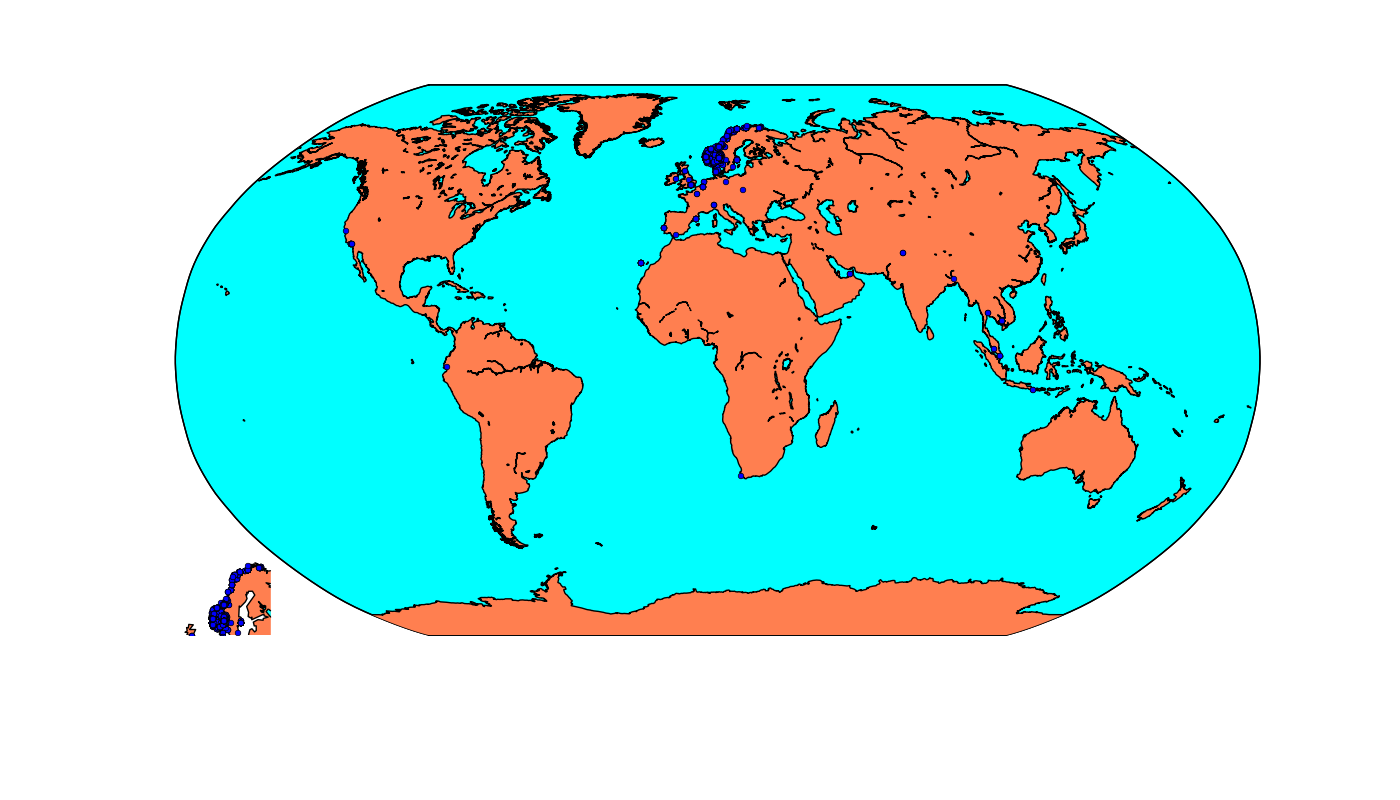
\includegraphics[width=5in]{image/simpleGeoPlotworld.png}
        \centering
        \caption[Event location mapped on the world]{This figure shows the location of the events from all over the world.
        For a cropped version with focus on Norway and the surrounding countries, refer to~\ref{figure:croppedGeoplot}}
    \end{figure}

    \begin{figure}[H]
        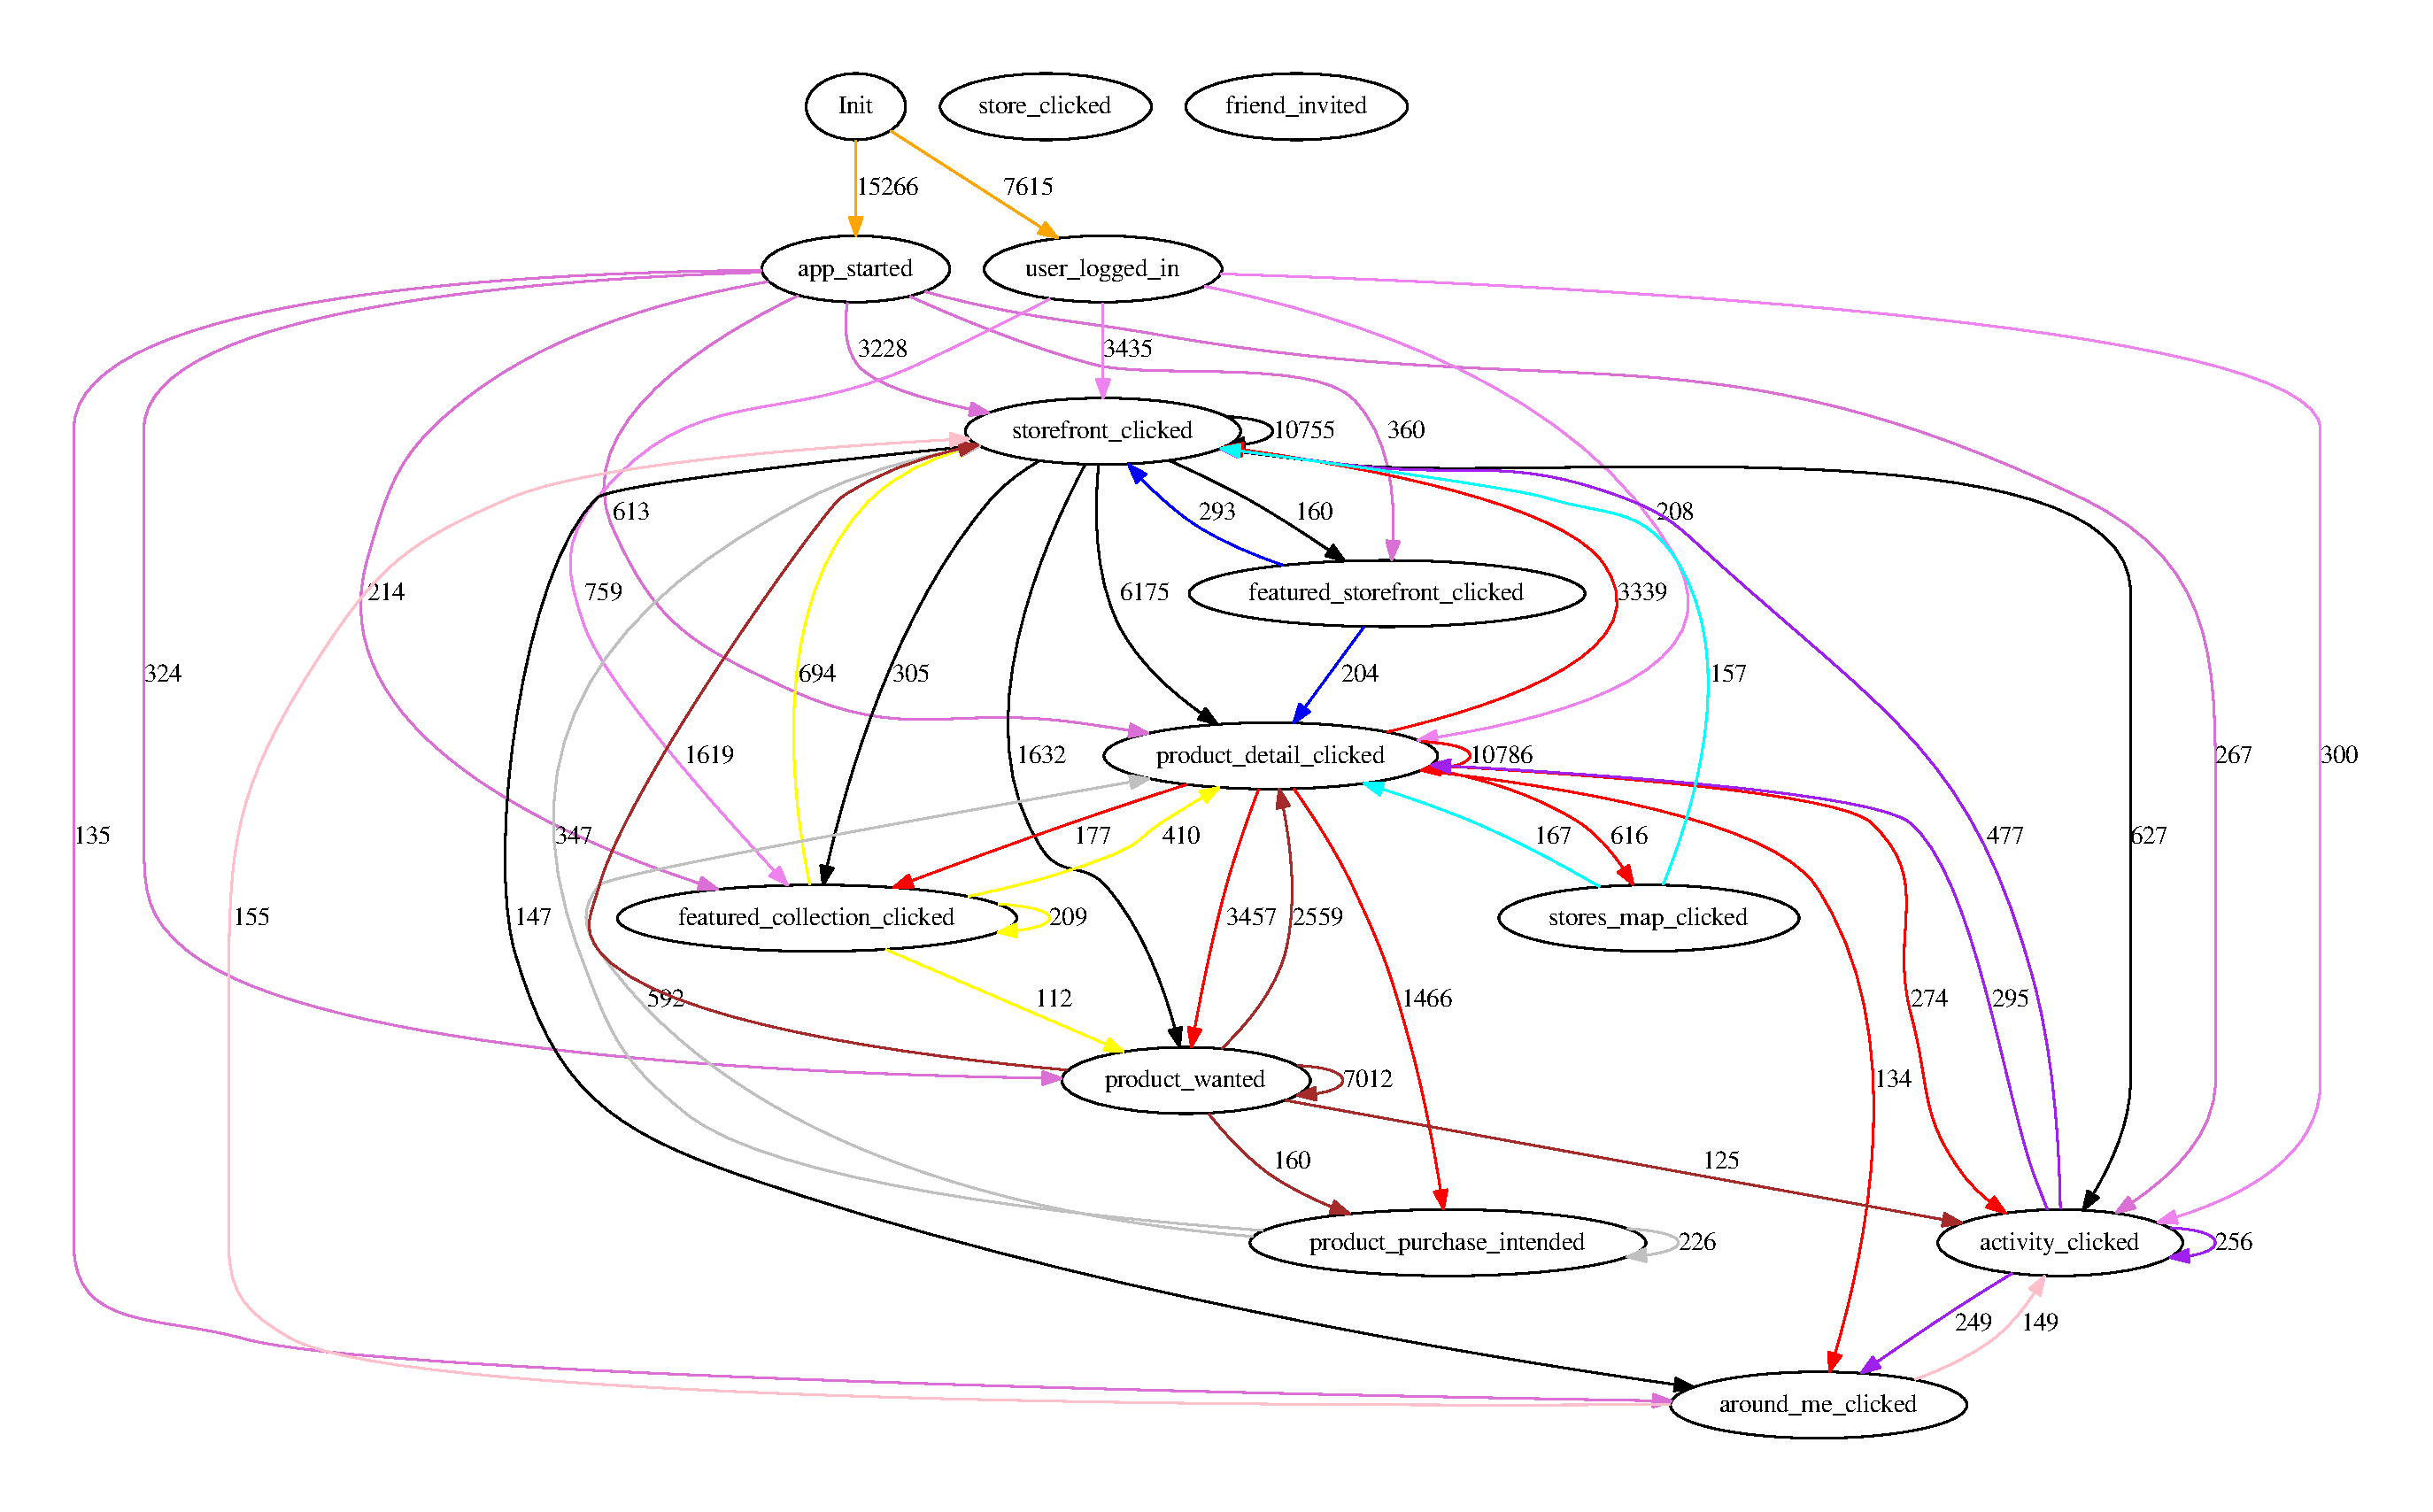
\includegraphics[width=5in]{image/statesInteractionFalse-gvfile.pdf}
        \centering
        \caption[States in session and how they interact]{The different states of the system and how they interact with each other.}
        \label{figure:statesInteractions}
    \end{figure}

\chapter{Extended State Of the Art}
\label{app:sota}

\section{Fashion domain}

\marginpar{TODO: Fix some kind of left align centering og content}
\begin{table}[H]
    \centering
    \begin{tabular}{ccc}
    \toprule
      \multicolumn{2}{c}{Concrete Attributes (Product Features)} & Abstract Attributes (Attitude-Based) \\
      \cmidrule(r{1em}){1-2}
      \multicolumn{1}{c}{Intrinsic (Hedonic)} & \multicolumn{1}{c}{Extrinsic} 				 	& \\ \midrule
      Style 				& Price						 	& Fun \\
      Color				& Brand 					 	& Entertainment \\
      Patten 				& Country of origin			 	& Enjoyment\\
      Fabric/fiber 		& Place(Store) 				 	& Need \\
      Appearance	   	 	& Salespeson's evaluation	 	&  Function\\
      Fashionability  	& Approval of others 		 	&\\
      Durability			& Coordination with wardrobe 	&\\
      Comfort				&								& \\
      Quality				&								& \\
      Fit					&								& \\
      Care 				&								& \\
    \bottomrule
    \end{tabular}
    \caption[Consumers' Purchase Decisions]{The attributes effecting the consumer when in the process of consuming products~\cite{dutton2006}}
    \label{table:ConsumersPurchaseDec}
\end{table}

\section{SoBazaar Competitors}\label{app:sec:soCompetitors}
\subsubsection{Flink} % (fold)
\label{par:flink}
    "Flink is THE brand-new app to discover, get inspired and share trendy looks from top fashion bloggers" - About Flink~\cite{flink}.

    Flink is a fashion discovery application for iPhone.
    It allows the user to browse fashion blogs, hot brands and new trends.

    The content displayed can be "liked" and can be a collection of clothes from different brands.
    If the user is interested in the item, the application can redirect the user to the web page where it is sold.
    \begin{table}[H]
            \centering
            \begin{tabularx}{\linewidth}{>{\parskip1ex}X@{\kern4\tabcolsep}>{\parskip1ex}X}
                \toprule
                \hfil\bfseries Strengths
                &
                \hfil\bfseries Weaknesses
                \\\cmidrule(r{3\tabcolsep}){1-1}\cmidrule(l{-\tabcolsep}){2-2}
                Can follow other users \par
                Connect with facebook \par
                Ability to add item to a \emph{want list} \par
                &
                No personalized recommendations \par
                \\\bottomrule
                \end{tabularx}
        \caption[Recommendation related strengths and weaknesses of Flink~\cite{flink}]{This table is the list of the recommendation related strengths and weaknesses of the mobile fashion application Flink~\cite{flink}}
        \label{table:iphoneAppFlink}
    \end{table}
  % todo - might be more, but can't explore the application since it is iOS 7 required
% paragraph flink (end)

\subsubsection{Motilo} % (fold)
\label{par:motilo}
    "Motilo was launched in 2011 to answer that perennial fashion dilemma all women face --- what shall I wear tonight?" - About Motilo~\cite{motilo}.

    Items on the web page are gathered by the Motilo stylists.
    This gives the page a fresh set of items for the user to select from.

    Motilo gives the user the ability to put together item sets through dragging and dropping the items into a "fashion dilemma", or simply like items.
    The user can ask friends, the Motilo community or the Motilo stylists about suggestions regarding what to wear.
    If the user wants to buy an item, Motilo redirects the user to the page which sells the item in question.

    \begin{table}[H]
    \centering
    \begin{tabularx}{\linewidth}{>{\parskip1ex}X@{\kern4\tabcolsep}>{\parskip1ex}X}
        \toprule
        \hfil\bfseries Strengths
        &
        \hfil\bfseries Weaknesses
            \\\cmidrule(r{3\tabcolsep}){1-1}\cmidrule(l{-\tabcolsep}){2-2}
            Connected with facebook \par
            Ability to add item to a "want list" \par
            A feed with the most trending item collections \par
            Ask Motilo stylists for suggestions \par
            &
            Manual/limited personalized recommendations \par
            \\\bottomrule
            \end{tabularx}
            \caption[Recommendation related strengths and weaknesses of Motilo~\cite{motilo}]{This table is the list of the recommendation related strengths and weaknesses of e-commerce fashion web site Motilo~\cite{motilo}}
            \label{table:ecommenreceMotilo}
        \end{table}
% paragraph motilo (end)


\subsubsection{ModCloth} % (fold)
\label{par:modcloth}
    "A top e-retailer of indie clothing, accessories, and decor, and provide an engaging shopping experience where you, our customer, can have a voice" - About ModCloth~\cite{modcloth}

    ModCloth focuses on giving what the community is looking for.
    The user is given the opportunity to both be the seller and the buyer.
    The item base is affected by the user trough voting.
    \begin{table}[H]
            \centering
            \begin{tabularx}{\linewidth}{>{\parskip1ex}X@{\kern4\tabcolsep}>{\parskip1ex}X}
                \toprule
                \hfil\bfseries Strengths
                &
                \hfil\bfseries Weaknesses
                \\\cmidrule(r{3\tabcolsep}){1-1}\cmidrule(l{-\tabcolsep}){2-2}
                Ability to add item to a "want list" \par
                A feed with the most popular items \par
                A feed with new items \par
                A list of similar items \par
                &
                No personalized recommendations \par
                \\ \bottomrule
        \end{tabularx}
        \caption[Recommendation related strengths and weaknesses of
        ModCloth~\cite{modcloth}]{This table is the list of the recommendation
        related strengths and weaknesses of e-commerce fashion web site
        ModCloth~\cite{modcloth}}
        \label{table:ecommenreceModCloth}
    \end{table}
% paragraph modcloth (end)

\subsubsection{UsTrendy} % (fold)
\label{par:ustrendy}
    "UsTrendy allows you to shop and discover one-of-a-kind fashions from all over the world." - About UsTrendy~\cite{UsTrendy}

    UsTrendy has a large item database of more than hundred thousand unique items.

    When the user is viewing an item, UsTrendy displays other items the user might like, which have common traits with the one the user is currently watching.
    The currently viewed item can be added to a sopping cart.
    \begin{table}[H]
                \centering
                \begin{tabularx}{\linewidth}{>{\parskip1ex}X@{\kern4\tabcolsep}>{\parskip1ex}X}
                    \toprule
                    \hfil\bfseries Strengths
                    &
                    \hfil\bfseries Weaknesses
                    \\\cmidrule(r{3\tabcolsep}){1-1}\cmidrule(l{-\tabcolsep}){2-2}
                  Ability to add item to a "want list" \par
                  A feed with the most popular items \par
                  A feed with new items \par
                  A list of similar items \par
                  &
                  No personalized recommendations \par
                \\ \bottomrule
        \end{tabularx}
        \caption[Recommendation related strengths and weaknesses of UsTrendy~\cite{UsTrendy}]{This table is the list of the recommendation related strengths and weaknesses of e-commerce fashion web site UsTrendy~\cite{UsTrendy}}
        \label{table:ecommenreceUsTrendy}
    \end{table}
% paragraph ustrendy (end)

\subsubsection{Polyvore} % (fold)
\label{par:polyvore}
    "Polyvore is a new way to discover and shop for things you love." - About Polyvore~\cite{polyvore}

    In Polyvore the user can put together sets of items and show them off to their friends and others.
    The items shown on Polyvore are gathered based on the community of Polyvore.

    When accessing an item the user is shown similar items to the one which is currently being watched.
    When the user want to purchase an item, the user is redirected to the page which sells the item.
    \begin{table}[H]
                \centering
                \begin{tabularx}{\linewidth}{>{\parskip1ex}X@{\kern4\tabcolsep}>{\parskip1ex}X}
                \toprule
                \hfil\bfseries Strengths
                &
                \hfil\bfseries Weaknesses
                \\\cmidrule(r{3\tabcolsep}){1-1}\cmidrule(l{-\tabcolsep}){2-2}
                    Ability to add item to a "want list" \par
                    The user can follow other users \par
                    Crawl other fashion sites to add to their item base \par
                    A feed with trending items \par
                    A list of recently viewed items \par
                &
                    No personalized recommendations \par
                \\ \bottomrule
        \end{tabularx}
        \caption[Recommendation related strengths and weaknesses of
        Polyvore~\cite{polyvore}]{This table is the list of the recommendation
        related strengths and weaknesses of e-commerce fashion web site
        Polyvore~\cite{polyvore}}
        \label{table:ecommenrecePolyvore}
    \end{table}
% paragraph polyvore (end)

\subsubsection{Clothia} % (fold)
\label{par:clothia}
    "An online destination where you can mix and match outfits, share looks you love, even try on clothes virtually via your webcam using augmented reality technology" - About Clothia~\cite{clothia}

    The user can put together a set of clothes from the web site and make a "set".
    The set can be shared with other users and like by other users.
    If the user is interested in buying an item, the user is redirected to the page from which the item is sold.
    \begin{table}[H]
                \centering
                \begin{tabularx}{\linewidth}{>{\parskip1ex}X@{\kern4\tabcolsep}>{\parskip1ex}X}
                \toprule
                \hfil\bfseries Strengths
                &
                \hfil\bfseries Weaknesses
                \\\cmidrule(r{3\tabcolsep}){1-1}\cmidrule(l{-\tabcolsep}){2-2}
                Ability to add item to a "want list" \par
                The user can follow other users \par
                A feed with trending items \par
                &
                Lack personalized recommendations \par
                \\ \bottomrule
        \end{tabularx}
        \caption[Recommendation related strengths and weaknesses of Clothia~\cite{clothia}]{This table is the list of the recommendation related strengths and weaknesses of e-commerce fashion web site Clothia~\cite{clothia}}
        \label{table:ecommenreceClothia}
    \end{table}
% paragraph clothia (end)

\subsubsection{Trendabl} % (fold)
\label{par:trendabl}
    "Trendabl is a community of people who love fashion" - About Trendable~\cite{trendabl}

    The user is shown a feed with the newest items, and is free to browse different sets of collections, such as collections with shoes and pants.
    If the user wants to buy an item it can be added to a shopping chart.
    \begin{table}[H]
                    \centering
                    \begin{tabularx}{\linewidth}{>{\parskip1ex}X@{\kern4\tabcolsep}>{\parskip1ex}X}
                    \toprule
                    \hfil\bfseries Strengths
                    &
                    \hfil\bfseries Weaknesses
                    \\\cmidrule(r{3\tabcolsep}){1-1}\cmidrule(l{-\tabcolsep}){2-2}
                    Ability to add item to a "want list" \par
                    The user can follow other users \par
                    System recommends the top users in the system for the user to follow \par
                    &
                    No personalized recommendations \par
                    \\ \bottomrule
        \end{tabularx}
        \caption[Recommendation related strengths and weaknesses of Trendabl~\cite{trendabl}]{This table is the list of the recommendation related strengths and weaknesses of e-commerce fashion web site Trendabl~\cite{trendabl}}
        \label{table:ecommenreceTrendabl}
    \end{table}
% paragraph trendabl (end)


\subsubsection{Rue La La} % (fold)
\label{par:rue_la_la}
    "Rue La La is the destination for the most desired brands" - About Rue La La~\cite{RueLaLa}

    Rue La La is a sale on site e-commerce web site.
    It is built up of a set of different boutiques, which can be browsed by the user.
    When the user is watching an item, Rue La La shows other items from the current boutique.

    \begin{table}[H]
                \centering
                \begin{tabularx}{\linewidth}{>{\parskip1ex}X@{\kern4\tabcolsep}>{\parskip1ex}X}
                \toprule
                \hfil\bfseries Strengths
                &
                \hfil\bfseries Weaknesses
                \\\cmidrule(r{3\tabcolsep}){1-1}\cmidrule(l{-\tabcolsep}){2-2}
                Ability to add item to a "want list" \par
                List of most popular items \par
                &
                No personalized recommendations \par
                \\ \bottomrule
        \end{tabularx}
        \caption[Recommendation related strengths and weaknesses of Rue La La~\cite{RueLaLa}]{This table is the list of the recommendation related strengths and weaknesses of e-commerce fashion web site Rue La La~\cite{RueLaLa}}
        \label{table:ecommenreceRueLaLa}
    \end{table}
% paragraph rue_la_la (end)

\subsubsection{Zalando} % (fold)
\label{par:zalando}
    "Clothes, accessories, sports items, beauty products" - About Zalando~\cite{Zalando}

    Zalando has a large set of items.
    When browsing an item the user is shown a set of similar items the user might also like, and a set of items which might "go well"  with the currently viewed item.

    \begin{table}[H]
                    \centering
                    \begin{tabularx}{\linewidth}{>{\parskip1ex}X@{\kern4\tabcolsep}>{\parskip1ex}X}
                    \toprule
                    \hfil\bfseries Strengths
                    &
                    \hfil\bfseries Weaknesses
                    \\\cmidrule(r{3\tabcolsep}){1-1}\cmidrule(l{-\tabcolsep}){2-2}
                    Ability to add item to a "want list" \par
                    Shop on site \par
                    Similar items \par
                    &
                    No personalized recommendations \par
                    \\ \bottomrule
        \end{tabularx}
        \caption[Recommendation related strengths and weaknesses of Zalando~\cite{Zalando}]{This table is the list of the recommendation related strengths and weaknesses of e-commerce fashion web site Zalando~\cite{Zalando}}
        \label{table:ecommenreceZalando}
    \end{table}
% paragraph zalando (end)

\subsubsection{Ellos~\cite{Ellos}} % (fold)
\label{par:ellos}
    Ellos is a e-commerce web site, which specializes in fashion.

    When browsing an item, similar items to the one currently being watched is presented to the user.
    Other items which might go well with the item is also presented for the user.

    \begin{table}[H]
                \centering
                \begin{tabularx}{\linewidth}{>{\parskip1ex}X@{\kern4\tabcolsep}>{\parskip1ex}X}
                \toprule
                \hfil\bfseries Strengths
                &
                \hfil\bfseries Weaknesses
                \\\cmidrule(r{3\tabcolsep}){1-1}\cmidrule(l{-\tabcolsep}){2-2}
                Ability to add item to a "want list" \par
                Shop on site \par
                Similar items \par
                On site most popular list \par
                Items which might go well with the current \par
                &
                No personalized recommendations \par
                \\ \bottomrule
        \end{tabularx}
        \caption[Recommendation related strengths and weaknesses of Ellos~\cite{Ellos}]{This table is the list of the recommendation related strengths and weaknesses of e-commerce fashion web site Ellos~\cite{Ellos}}
        \label{table:ecommenreceEllos}
    \end{table}
% paragraph ellos (end)

\subsubsection{LookBook} % (fold)
\label{par:lookbook}
    "LOOKBOOK is the \#1 source for fashion inspiration from real people around the world." - About LookBook~\cite{LookBook}

    LookBook is a leading online community which is centered around the looks of the users.
    The users can share their own looks and keep up with other users through watching their uploads.
    With over 1.2 million members LookBook is constantly up to date on the newest fashion trends.
    \begin{table}[H]
                \centering
                \begin{tabularx}{\linewidth}{>{\parskip1ex}X@{\kern4\tabcolsep}>{\parskip1ex}X}
                \toprule
                \hfil\bfseries Strengths
                &
                \hfil\bfseries Weaknesses
                \\\cmidrule(r{3\tabcolsep}){1-1}\cmidrule(l{-\tabcolsep}){2-2}
                Ability to add item to a "want list" \par
                Shop on site \par
                Similar items \par
                Most popular items list \par
                Hot items list \par
                &
                No personalized recommendations \par
                \\ \bottomrule
        \end{tabularx}
        \caption[Recommendation related strengths and weaknesses of LookBook~\cite{LookBook}]{This table is the list of the recommendation related strengths and weaknesses of e-commerce fashion web site LookBook~\cite{LookBook}}
        \label{table:ecommenreceLookBook}
    \end{table}
% paragraph lookbook (end)


\subsubsection{Fashiolista} % (fold)
\label{par:fashiolista}
    "Let Fashiolista's community be your style guide in the online fashion jungle" - About Fasho~\cite{Fashiolista}

    The items on Fashiolista is selected by the users of Fashiolista, and the sites is therefore customized to fit the user crowd's wishes and interests.

    When accessing an item, the user is presented with the item, and a set of other items from the store the current item originated from.
    Other users who liked the item are also shown, so the user can browse their personal want list.
    \begin{table}[H]
                    \centering
                    \begin{tabularx}{\linewidth}{>{\parskip1ex}X@{\kern4\tabcolsep}>{\parskip1ex}X}
                    \toprule
                    \hfil\bfseries Strengths
                    &
                    \hfil\bfseries Weaknesses
                    \\\cmidrule(r{3\tabcolsep}){1-1}\cmidrule(l{-\tabcolsep}){2-2}
                Ability to add item to a "want list" \par
                On site most popular list \par
             &
                 No personalized recommendations \par
             \\ \bottomrule
        \end{tabularx}
        \caption[Recommendation related strengths and weaknesses of Fashiolista~\cite{Fashiolista}]{This table is the list of the recommendation related strengths and weaknesses of e-commerce fashion web site Fashiolista~\cite{Fashiolista}}
        \label{table:ecommenreceFahiolista}
    \end{table}
% paragraph fashiolista (end)

\subsubsection{ShopStyle} % (fold)
\label{par:shopstyle}
    "POPSUGAR is a global women's lifestyle brand focused in media, commerce, and technology" - About ShopStyle~\cite{ShopStyle}

    ShopStyle is a commerce brand of POPSUGAR.
    ShopStyle displays items from other e-commerce web sites, and redirects the user directly to the e-commerce web site from which the item clicked originated.
    Items can be liked on ShopStyle, and viewed in less detail at the web page of ShopStyle.
    \begin{table}[H]
                    \centering
                    \begin{tabularx}{\linewidth}{>{\parskip1ex}X@{\kern4\tabcolsep}>{\parskip1ex}X}
                    \toprule
                    \hfil\bfseries Strengths
                    &
                    \hfil\bfseries Weaknesses
                    \\\cmidrule(r{3\tabcolsep}){1-1}\cmidrule(l{-\tabcolsep}){2-2}
                Ability to add item to a "want list" \par
                Similar items \par
                Editor's picks \par
            &
                No personalized recommendations \par
            \\ \bottomrule
        \end{tabularx}
        \caption[Recommendation related strengths and weaknesses of ShopStyle~\cite{ShopStyle}]{This table is the list of the recommendation related strengths and weaknesses of e-commerce fashion web site ShopStyle~\cite{ShopStyle}}
        \label{table:ecommenreceShopStyle}
    \end{table}
% paragraph shopstyle (end)

\section{State of the Art: Evaluation}
\label{appendix:evaluation-metrics}

% Describe why this is in the Appendix.
In this section we will cover an in-depth study of evaluation metrics and
methods, which were not included in~\ref{sec:evaluation} as they are not
directly suited for either the domain or setting in the proposed system.
They are included here as they may provide clarity on \textit{why} they are not
suited, as well the fact that non-suitednes is a result in itself. Finally we
identify some resources of which the avid reader may do further research into
the field of evaluation recommender systems.

% Boostrapping in Appendix, as we do not use it and Helge proposed it.
\subsubsection{Using bootstrapping for validating offline experiments}
Bootstrapping~\cite{efron1994introduction} is used to estimate properties of an
estimate, such as bias, variance, confidence, intervals and prediction error.
This is done trough measuring these properties when sampling from an
approximated distribution, creating an empirical distribution of the observed
data.  Since the entire population is unknown it will not be possible to
calculate the true error from the sample data.  The idea then is that with this
information from sample data it is possible to say something about the
population.  Since it will not be possible to perform inference on:

\emph{sample data} $\rightarrow$ \emph{population} this is modeled as:
\emph{re-sample data} $\rightarrow$ \emph{sample data}.
The \emph{re-sample data} is a re-sampling of the sample data.

In practice an example to bootstrapping is when we want to calculate the
average height of the population worldwide.  The issue here is that it is not
as doable to measure everyone, so a subset of the population is used.  Since
the average on this number only will be an estimate of the actual world wide
average a sense of error margin must be introduced.  Bootstrapping is then used
to reduce the error of margin through re-sampling the sample data a large
number of times~\footnote{Numbers vary on sample size, but is often 1 000 to 10
000}, and new averages are calculated.  With these averages a histogram can be
produced, which provides an estimate of the distribution of this average.

\begin{figure}[H]
    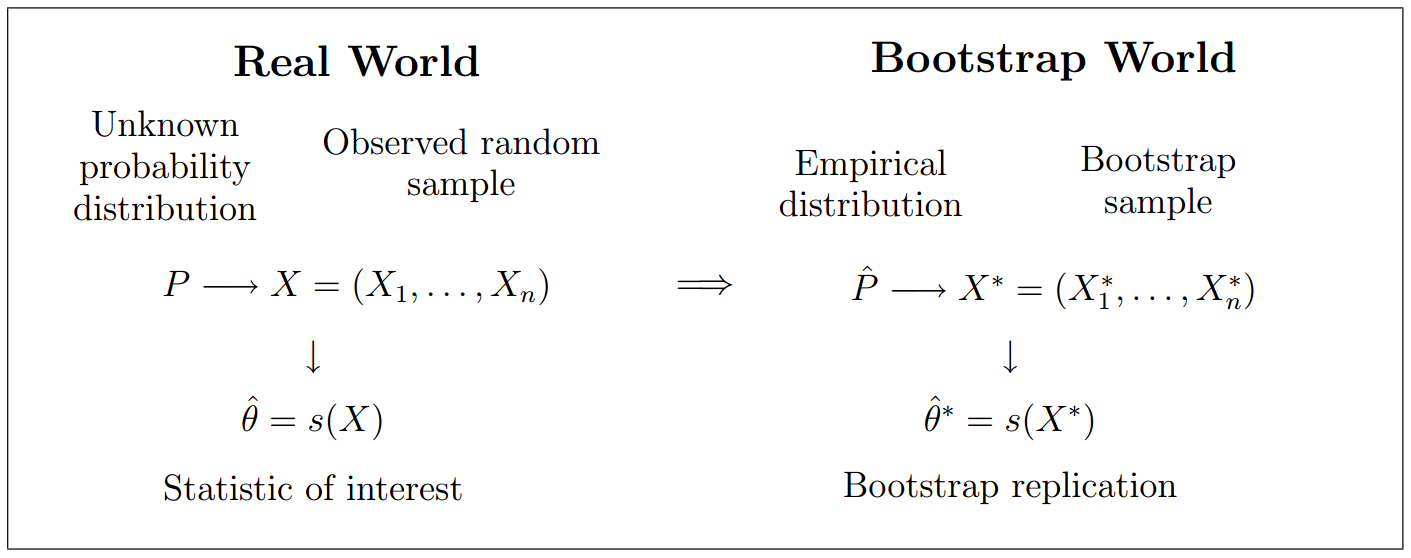
\includegraphics[scale=0.6]{image/bootstrap.png}
    \centering
    \caption[Bootstrapping principles]{A figure of the principles bootstrapping. Taken from~\cite{Eichler2003}}
    \label{figure:bootstrapping}
\end{figure}

One prominent issue with bootstrapping is that important properties of the
actual data might not be caught when undertaking the bootstrapping analysis
~\footnote{"Bootstrapping" comes from the phrase, "to pull oneself up by one's
bootstraps"~\cite{bootstrapSaying1843}}.

% Sub-section on resources available for avid readers who want further research
% into the field of evaluating recommender systems.
\subsubsection{Datasets for Offline Evaluation}
The main aim of a recommender system is to identify the set of items in a
dataset that might be interesting to a user based on their expressed
preferences. For a fashion recommender this would mean estimating how much a
user might like an item, by e.g.\\ predicting what rating a user might give an
item. In recent years, various test collections for different domains such as
books, music, movies have been made available to the public. These datasets
usually consist of user ratings similar to the ones used in this thesis (see
Section~\ref{}):

\begin{table}[H]
\centering
	\begin{tabular}{*{4}l}
	\toprule
		User ID & Item ID & Rating & Timestamp \\ \midrule
		1		  &	11	  &	5	    &  2014-12-15 10:14:51  \\
		2		  &	19	  &	2	    &  2014-12-12 11:44:31  \\
		\dots &	\dots &	\dots &  \dots                \\
	\bottomrule
	\end{tabular}
\caption{Classical recommender system dataset}
\end{table}

In recent years more or more datasets have been made available which contains
additional information such as demographic information about the users,
trust-networks, user-assigned tags and etc. Below we have listed a few selected
popular datasets containing additional information:

\begin{itemize}

\item \textbf{MovieLens 100k dataset}~\cite{Movielens}: The movielens dataset
	incorporates demographic information about the user in addition the
	traditional rating matrix

\item \textbf{Epinions dataset}~\cite{Epinions}: The Epinions dataset includes a
	trust-network, which specifices who-trust-whom in a social network based on
	customer reviews for the website Epinions.com

\item \textbf{The Million Song Dataset}~\cite{Bertin-Mahieux2011}: The million song
	dataset is a implicit feedback dataset. This data also includes information on the users,
	and audio features and song meta-data.

\item \textbf{The Book-Crossing Dataset}: The bookcrossing dataset consists of both implicit and explicit feedback,
	demographic information about users and some content based information about the books.
\end{itemize}

\chapter{Extended Implementation}
\label{app:impl}

\section{Implemented Functional Requirements}
\begin{enumerate}[label=\bfseries FR \arabic*:]
  \item {\color{ForestGreen}Blablaba}
  \item {\color{RedOrange}\st{Blablaba}}
\end{enumerate}

\section{Implemented Non Functional Requirements}
\begin{enumerate}[label=\bfseries NFR \arabic*:]
  \item {\color{ForestGreen}Blablaba}
  \item {\color{RedOrange}\st{Blablaba}}
\end{enumerate}

\section{Experimental Results}
\label{app:results}


%----------------------------------------------
% BIBLIOGRAPHY
%----------------------------------------------
\clearpage
\addcontentsline{toc}{chapter}{References}
\bibliographystyle{plain}
\bibliography{references}

\end{document}
